%%%%%%%%%%%%%%%%%%%%%%%%%%%%%%%%%%%%%%%%%
% The Legrand Orange Book
% LaTeX Template
% Version 2.0 (9/2/15)
%
% This template has been downloaded from:
% http://www.LaTeXTemplates.com
%
% Mathias Legrand (legrand.mathias@gmail.com) with modifications by:
% Vel (vel@latextemplates.com)
%
% License:
% CC BY-NC-SA 3.0 (http://creativecommons.org/licenses/by-nc-sa/3.0/)
%
% Compiling this template:
% This template uses biber for its bibliography and makeindex for its index.
% When you first open the template, compile it from the command line with the 
% commands below to make sure your LaTeX distribution is configured correctly:
%
% 1) pdflatex main
% 2) makeindex main.idx -s StyleInd.ist
% 3) biber main
% 4) pdflatex main x 2
%
% After this, when you wish to update the bibliography/index use the appropriate
% command above and make sure to compile with pdflatex several times 
% afterwards to propagate your changes to the document.
%
% This template also uses a number of packages which may need to be
% updated to the newest versions for the template to compile. It is strongly
% recommended you update your LaTeX distribution if you have any
% compilation errors.
%
% Important note:
% Chapter heading images should have a 2:1 width:height ratio,
% e.g. 920px width and 460px height.
%
%%%%%%%%%%%%%%%%%%%%%%%%%%%%%%%%%%%%%%%%%

%----------------------------------------------------------------------------------------
%	PACKAGES AND OTHER DOCUMENT CONFIGURATIONS
%----------------------------------------------------------------------------------------

\documentclass[11pt,fleqn]{book} % Default font size and left-justified equations

%----------------------------------------------------------------------------------------

%%%%%%%%%%%%%%%%%%%%%%%%%%%%%%%%%%%%%%%%%
% The Legrand Orange Book
% Structural Definitions File
% Version 2.0 (9/2/15)
%
% Original author:
% Mathias Legrand (legrand.mathias@gmail.com) with modifications by:
% Vel (vel@latextemplates.com)
% 
% This file has been downloaded from:
% http://www.LaTeXTemplates.com
%
% License:
% CC BY-NC-SA 3.0 (http://creativecommons.org/licenses/by-nc-sa/3.0/)
%
%%%%%%%%%%%%%%%%%%%%%%%%%%%%%%%%%%%%%%%%%

%----------------------------------------------------------------------------------------
%	VARIOUS REQUIRED PACKAGES AND CONFIGURATIONS
%----------------------------------------------------------------------------------------

\usepackage[top=3cm,bottom=3cm,left=3cm,right=3cm,headsep=10pt,a4paper]{geometry} % Page margins

\usepackage[table,xcdraw]{xcolor} % Required for specifying colors by name
\definecolor{ocre}{RGB}{243,102,25} % Define the orange color used for highlighting throughout the book
\definecolor{rightexample}{RGB}{31,181,0}
\definecolor{wrongexample}{RGB}{238,41,18}

% Used for longtables
\usepackage{tabularx}
\usepackage{longtable}
\usepackage{ltxtable}

\usepackage{graphicx} % Required for including pictures
\graphicspath{{Pictures/}} % Specifies the directory where pictures are stored

\usepackage{placeins} % Required for floatbarrier

\usepackage{lipsum} % Inserts dummy text

\usepackage{tikz} % Required for drawing custom shapes

\usepackage[english]{babel} % English language/hyphenation

\usepackage{enumitem} % Customize lists
\setlist{nolistsep} % Reduce spacing between bullet points and numbered lists

\usepackage{booktabs} % Required for nicer horizontal rules in tables

\usepackage{todonotes} % Used in order to make todos

\usepackage{xspace} % Used to make space in commands

% Used for making multiple figures within one figure
\usepackage{wrapfig}
\usepackage{subcaption}

\usepackage{array}

%----------------------------------------------------------------------------------------
%	FONTS
%----------------------------------------------------------------------------------------

\usepackage{avant} % Use the Avantgarde font for headings
%\usepackage{times} % Use the Times font for headings
\usepackage{mathptmx} % Use the Adobe Times Roman as the default text font together with math symbols from the Sym­bol, Chancery and Com­puter Modern fonts

\usepackage{microtype} % Slightly tweak font spacing for aesthetics
\usepackage[utf8]{inputenc} % Required for including letters with accents
\usepackage[T1]{fontenc} % Use 8-bit encoding that has 256 glyphs

%----------------------------------------------------------------------------------------
%	BIBLIOGRAPHY AND INDEX
%----------------------------------------------------------------------------------------

\usepackage[style=alphabetic,citestyle=numeric,sorting=nyt,sortcites=true,autopunct=true,babel=hyphen,hyperref=true,abbreviate=false,backref=true,backend=biber]{biblatex}
\addbibresource{bibliography.bib} % BibTeX bibliography file
\defbibheading{bibempty}{}

\usepackage{calc} % For simpler calculation - used for spacing the index letter headings correctly
\usepackage{makeidx} % Required to make an index
\makeindex % Tells LaTeX to create the files required for indexing

%----------------------------------------------------------------------------------------
%	MAIN TABLE OF CONTENTS
%----------------------------------------------------------------------------------------

\usepackage{titletoc} % Required for manipulating the table of contents

\contentsmargin{0cm} % Removes the default margin

% Part text styling
\titlecontents{part}[0cm]
{\addvspace{20pt}\centering\large\bfseries}
{}
{}
{}

% Chapter text styling
\titlecontents{chapter}[1.25cm] % Indentation
{\addvspace{12pt}\large\sffamily\bfseries} % Spacing and font options for chapters
{\color{ocre!60}\contentslabel[\Large\thecontentslabel]{1.25cm}\color{ocre}} % Chapter number
{\color{ocre}}  
{\color{ocre!60}\normalsize\;\titlerule*[.5pc]{.}\;\thecontentspage} % Page number

% Section text styling
\titlecontents{section}[1.25cm] % Indentation
{\addvspace{3pt}\sffamily\bfseries} % Spacing and font options for sections
{\contentslabel[\thecontentslabel]{1.25cm}} % Section number
{}
{\hfill\color{black}\thecontentspage} % Page number
[]

% Subsection text styling
\titlecontents{subsection}[1.25cm] % Indentation
{\addvspace{1pt}\sffamily\small} % Spacing and font options for subsections
{\contentslabel[\thecontentslabel]{1.25cm}} % Subsection number
{}
{\ \titlerule*[.5pc]{.}\;\thecontentspage} % Page number
[]

% List of figures
\titlecontents{figure}[0em]
{\addvspace{-5pt}\sffamily}
{\thecontentslabel\hspace*{1em}}
{}
{\ \titlerule*[.5pc]{.}\;\thecontentspage}
[]

% List of tables
\titlecontents{table}[0em]
{\addvspace{-5pt}\sffamily}
{\thecontentslabel\hspace*{1em}}
{}
{\ \titlerule*[.5pc]{.}\;\thecontentspage}
[]

%----------------------------------------------------------------------------------------
%	MINI TABLE OF CONTENTS IN PART HEADS
%----------------------------------------------------------------------------------------

% Chapter text styling
\titlecontents{lchapter}[0em] % Indenting
{\addvspace{15pt}\large\sffamily\bfseries} % Spacing and font options for chapters
{\color{ocre}\contentslabel[\Large\thecontentslabel]{1.25cm}\color{ocre}} % Chapter number
{}  
{\color{ocre}\normalsize\sffamily\bfseries\;\titlerule*[.5pc]{.}\;\thecontentspage} % Page number

% Section text styling
\titlecontents{lsection}[0em] % Indenting
{\sffamily\small} % Spacing and font options for sections
{\contentslabel[\thecontentslabel]{1.25cm}} % Section number
{}
{}

% Subsection text styling
\titlecontents{lsubsection}[.5em] % Indentation
{\normalfont\footnotesize\sffamily} % Font settings
{}
{}
{}

%----------------------------------------------------------------------------------------
%	PAGE HEADERS
%----------------------------------------------------------------------------------------

\usepackage{fancyhdr} % Required for header and footer configuration

\pagestyle{fancy}
\renewcommand{\chaptermark}[1]{\markboth{\sffamily\normalsize\bfseries\chaptername\ \thechapter.\ #1}{}} % Chapter text font settings
\renewcommand{\sectionmark}[1]{\markright{\sffamily\normalsize\thesection\hspace{5pt}#1}{}} % Section text font settings
\fancyhf{} \fancyhead[LE,RO]{\sffamily\normalsize\thepage} % Font setting for the page number in the header
\fancyhead[LO]{\rightmark} % Print the nearest section name on the left side of odd pages
\fancyhead[RE]{\leftmark} % Print the current chapter name on the right side of even pages
\renewcommand{\headrulewidth}{0.5pt} % Width of the rule under the header
\addtolength{\headheight}{2.5pt} % Increase the spacing around the header slightly
\renewcommand{\footrulewidth}{0pt} % Removes the rule in the footer
\fancypagestyle{plain}{\fancyhead{}\renewcommand{\headrulewidth}{0pt}} % Style for when a plain pagestyle is specified

% Removes the header from odd empty pages at the end of chapters
\makeatletter
\renewcommand{\cleardoublepage}{
\clearpage\ifodd\c@page\else
\hbox{}
\vspace*{\fill}
\thispagestyle{empty}
\newpage
\fi}

%----------------------------------------------------------------------------------------
%	THEOREM STYLES
%----------------------------------------------------------------------------------------

\usepackage{amsmath,amsfonts,amssymb,amsthm} % For math equations, theorems, symbols, etc

\newcommand{\intoo}[2]{\mathopen{]}#1\,;#2\mathclose{[}}
\newcommand{\ud}{\mathop{\mathrm{{}d}}\mathopen{}}
\newcommand{\intff}[2]{\mathopen{[}#1\,;#2\mathclose{]}}
\newtheorem{notation}{Notation}[chapter]

% Boxed/framed environments
\newtheoremstyle{ocrenumbox}% % Theorem style name
{0pt}% Space above
{0pt}% Space below
{\normalfont}% % Body font
{}% Indent amount
{\small\bf\sffamily\color{ocre}}% % Theorem head font
{\;}% Punctuation after theorem head
{0.25em}% Space after theorem head
{\small\sffamily\color{ocre}\thmname{#1}\nobreakspace\thmnumber{\@ifnotempty{#1}{}\@upn{#2}}% Theorem text (e.g. Theorem 2.1)
\thmnote{\nobreakspace\the\thm@notefont\sffamily\bfseries\color{black}---\nobreakspace#3.}} % Optional theorem note
\renewcommand{\qedsymbol}{$\blacksquare$}% Optional qed square

\newtheoremstyle{blacknumex}% Theorem style name
{5pt}% Space above
{5pt}% Space below
{\normalfont}% Body font
{} % Indent amount
{\small\bf\sffamily}% Theorem head font
{\;}% Punctuation after theorem head
{0.25em}% Space after theorem head
{\small\sffamily{\tiny\ensuremath{\blacksquare}}\nobreakspace\thmname{#1}\nobreakspace\thmnumber{\@ifnotempty{#1}{}\@upn{#2}}% Theorem text (e.g. Theorem 2.1)
\thmnote{\nobreakspace\the\thm@notefont\sffamily\bfseries---\nobreakspace#3.}}% Optional theorem note

\newtheoremstyle{blacknumbox} % Theorem style name
{0pt}% Space above
{0pt}% Space below
{\normalfont}% Body font
{}% Indent amount
{\small\bf\sffamily}% Theorem head font
{\;}% Punctuation after theorem head
{0.25em}% Space after theorem head
{\small\sffamily\thmname{#1}\nobreakspace\thmnumber{\@ifnotempty{#1}{}\@upn{#2}}% Theorem text (e.g. Theorem 2.1)
\thmnote{\nobreakspace\the\thm@notefont\sffamily\bfseries---\nobreakspace#3.}}% Optional theorem note

% Non-boxed/non-framed environments
\newtheoremstyle{ocrenum}% % Theorem style name
{5pt}% Space above
{5pt}% Space below
{\normalfont}% % Body font
{}% Indent amount
{\small\bf\sffamily\color{ocre}}% % Theorem head font
{\;}% Punctuation after theorem head
{0.25em}% Space after theorem head
{\small\sffamily\color{ocre}\thmname{#1}\nobreakspace\thmnumber{\@ifnotempty{#1}{}\@upn{#2}}% Theorem text (e.g. Theorem 2.1)
\thmnote{\nobreakspace\the\thm@notefont\sffamily\bfseries\color{black}---\nobreakspace#3.}} % Optional theorem note
\renewcommand{\qedsymbol}{$\blacksquare$}% Optional qed square
\makeatother

% Defines the theorem text style for each type of theorem to one of the three styles above
\newcounter{dummy} 
\numberwithin{dummy}{section}
\theoremstyle{ocrenumbox}
\newtheorem{theoremeT}[dummy]{Theorem}
\newtheorem{problem}{Problem}[chapter]
\newtheorem{exerciseT}{Exercise}[chapter]
\theoremstyle{blacknumex}
\newtheorem{exampleT}{Example}[chapter]
\theoremstyle{blacknumbox}
\newtheorem{vocabulary}{Vocabulary}[chapter]
\newtheorem{definitionT}{Definition}[section]
\newtheorem{corollaryT}[dummy]{Corollary}
\newtheorem{noteT}[dummy]{Note}
\theoremstyle{ocrenum}
\newtheorem{proposition}[dummy]{Proposition}

%----------------------------------------------------------------------------------------
%	DEFINITION OF COLORED BOXES
%----------------------------------------------------------------------------------------

\RequirePackage[framemethod=default]{mdframed} % Required for creating the theorem, definition, exercise and corollary boxes

% Theorem box
\newmdenv[skipabove=7pt,
skipbelow=7pt,
backgroundcolor=black!5,
linecolor=ocre,
innerleftmargin=5pt,
innerrightmargin=5pt,
innertopmargin=5pt,
leftmargin=0cm,
rightmargin=0cm,
innerbottommargin=5pt]{tBox}

% Exercise box	  
\newmdenv[skipabove=7pt,
skipbelow=7pt,
rightline=false,
leftline=true,
topline=false,
bottomline=false,
backgroundcolor=ocre!10,
linecolor=ocre,
innerleftmargin=5pt,
innerrightmargin=5pt,
innertopmargin=5pt,
innerbottommargin=5pt,
leftmargin=0cm,
rightmargin=0cm,
linewidth=4pt]{eBox}

% Example box (Right)	  
\newmdenv[skipabove=7pt,
skipbelow=7pt,
rightline=false,
leftline=true,
topline=false,
bottomline=false,
backgroundcolor=rightexample!10,
linecolor=rightexample,
innerleftmargin=5pt,
innerrightmargin=5pt,
innertopmargin=5pt,
innerbottommargin=5pt,
leftmargin=0cm,
rightmargin=0cm,
linewidth=4pt]{erBox}

% Example box (Wrong)	  
\newmdenv[skipabove=7pt,
skipbelow=7pt,
rightline=false,
leftline=true,
topline=false,
bottomline=false,
backgroundcolor=wrongexample!10,
linecolor=wrongexample,
innerleftmargin=5pt,
innerrightmargin=5pt,
innertopmargin=5pt,
innerbottommargin=5pt,
leftmargin=0cm,
rightmargin=0cm,
linewidth=4pt]{ewBox}

% Definition box
\newmdenv[skipabove=7pt,
skipbelow=7pt,
rightline=false,
leftline=true,
topline=false,
bottomline=false,
linecolor=ocre,
innerleftmargin=5pt,
innerrightmargin=5pt,
innertopmargin=0pt,
leftmargin=0cm,
rightmargin=0cm,
linewidth=4pt,
innerbottommargin=0pt]{dBox}	

% Corollary box
\newmdenv[skipabove=7pt,
skipbelow=7pt,
rightline=false,
leftline=true,
topline=false,
bottomline=false,
linecolor=gray,
backgroundcolor=black!5,
innerleftmargin=5pt,
innerrightmargin=5pt,
innertopmargin=5pt,
leftmargin=0cm,
rightmargin=0cm,
linewidth=4pt,
innerbottommargin=5pt]{cBox}

% Note box
\newmdenv[skipabove=7pt,
skipbelow=7pt,
rightline=false,
leftline=true,
topline=false,
bottomline=false,
linecolor=gray,
backgroundcolor=black!5,
innerleftmargin=5pt,
innerrightmargin=5pt,
innertopmargin=5pt,
leftmargin=0cm,
rightmargin=0cm,
linewidth=4pt,
innerbottommargin=5pt]{nBox}

% Creates an environment for each type of theorem and assigns it a theorem text style from the "Theorem Styles" section above and a colored box from above
\newenvironment{theorem}{\begin{tBox}\begin{theoremeT}}{\end{theoremeT}\end{tBox}}
\newenvironment{exercise}{\begin{eBox}\begin{exerciseT}}{\hfill{\color{ocre}\tiny\ensuremath{\blacksquare}}\end{exerciseT}\end{eBox}}

\newenvironment{exampleR}{\begin{erBox}\begin{exampleT}}{\hfill{\color{ocre}\tiny}\end{exampleT}\end{erBox}}

\newenvironment{exampleW}{\begin{ewBox}\begin{exampleT}}{\hfill{\color{ocre}\tiny}\end{exampleT}\end{ewBox}}

\newenvironment{definition}{\begin{dBox}\begin{definitionT}}{\end{definitionT}\end{dBox}}	
\newenvironment{example}{\begin{exampleT}}{\hfill{\tiny\ensuremath{\blacksquare}}\end{exampleT}}		
\newenvironment{corollary}{\begin{cBox}\begin{corollaryT}}{\end{corollaryT}\end{cBox}}

\newenvironment{note}{\begin{nBox}\begin{noteT}}{\end{noteT}\end{nBox}}	

%----------------------------------------------------------------------------------------
%	REMARK ENVIRONMENT
%----------------------------------------------------------------------------------------

\newenvironment{remark}{\par\vspace{10pt}\small % Vertical white space above the remark and smaller font size
\begin{list}{}{
\leftmargin=35pt % Indentation on the left
\rightmargin=25pt}\item\ignorespaces % Indentation on the right
\makebox[-2.5pt]{\begin{tikzpicture}[overlay]
\node[draw=ocre!60,line width=1pt,circle,fill=ocre!25,font=\sffamily\bfseries,inner sep=2pt,outer sep=0pt] at (-15pt,0pt){\textcolor{ocre}{R}};\end{tikzpicture}} % Orange R in a circle
\advance\baselineskip -1pt}{\end{list}\vskip5pt} % Tighter line spacing and white space after remark

%----------------------------------------------------------------------------------------
%	SECTION NUMBERING IN THE MARGIN
%----------------------------------------------------------------------------------------

\makeatletter
\renewcommand{\@seccntformat}[1]{\llap{\textcolor{ocre}{\csname the#1\endcsname}\hspace{1em}}}                    
\renewcommand{\section}{\@startsection{section}{1}{\z@}
{-4ex \@plus -1ex \@minus -.4ex}
{1ex \@plus.2ex }
{\normalfont\large\sffamily\bfseries}}
\renewcommand{\subsection}{\@startsection {subsection}{2}{\z@}
{-3ex \@plus -0.1ex \@minus -.4ex}
{0.5ex \@plus.2ex }
{\normalfont\sffamily\bfseries}}
\renewcommand{\subsubsection}{\@startsection {subsubsection}{3}{\z@}
{-2ex \@plus -0.1ex \@minus -.2ex}
{.2ex \@plus.2ex }
{\normalfont\small\sffamily\bfseries}}                        
\renewcommand\paragraph{\@startsection{paragraph}{4}{\z@}
{-2ex \@plus-.2ex \@minus .2ex}
{.1ex}
{\normalfont\small\sffamily\bfseries}}

%----------------------------------------------------------------------------------------
%	PART HEADINGS
%----------------------------------------------------------------------------------------

% numbered part in the table of contents
\newcommand{\@mypartnumtocformat}[2]{%
\setlength\fboxsep{0pt}%
\noindent\colorbox{ocre!20}{\strut\parbox[c][.7cm]{\ecart}{\color{ocre!70}\Large\sffamily\bfseries\centering#1}}\hskip\esp\colorbox{ocre!40}{\strut\parbox[c][.7cm]{\linewidth-\ecart-\esp}{\Large\sffamily\centering#2}}}%
%%%%%%%%%%%%%%%%%%%%%%%%%%%%%%%%%%
% unnumbered part in the table of contents
\newcommand{\@myparttocformat}[1]{%
\setlength\fboxsep{0pt}%
\noindent\colorbox{ocre!40}{\strut\parbox[c][.7cm]{\linewidth}{\Large\sffamily\centering#1}}}%
%%%%%%%%%%%%%%%%%%%%%%%%%%%%%%%%%%
\newlength\esp
\setlength\esp{4pt}
\newlength\ecart
\setlength\ecart{1.2cm-\esp}
\newcommand{\thepartimage}{}%
\newcommand{\partimage}[1]{\renewcommand{\thepartimage}{#1}}%
\def\@part[#1]#2{%
\ifnum \c@secnumdepth >-2\relax%
\refstepcounter{part}%
\addcontentsline{toc}{part}{\texorpdfstring{\protect\@mypartnumtocformat{\thepart}{#1}}{\partname~\thepart\ ---\ #1}}
\else%
\addcontentsline{toc}{part}{\texorpdfstring{\protect\@myparttocformat{#1}}{#1}}%
\fi%
\startcontents%
\markboth{}{}%
{\thispagestyle{empty}%
\begin{tikzpicture}[remember picture,overlay]%
\node at (current page.north west){\begin{tikzpicture}[remember picture,overlay]%	
\fill[ocre!20](0cm,0cm) rectangle (\paperwidth,-\paperheight);
\node[anchor=north] at (4cm,-3.25cm){\color{ocre!40}\fontsize{220}{100}\sffamily\bfseries\@Roman\c@part}; 
\node[anchor=south east] at (\paperwidth-1cm,-\paperheight+1cm){\parbox[t][][t]{8.5cm}{
\printcontents{l}{0}{\setcounter{tocdepth}{1}}%
}};
\node[anchor=north east] at (\paperwidth-1.5cm,-3.25cm){\parbox[t][][t]{15cm}{\strut\raggedleft\color{white}\fontsize{30}{30}\sffamily\bfseries#2}};
\end{tikzpicture}};
\end{tikzpicture}}%
\@endpart}
\def\@spart#1{%
\startcontents%
\phantomsection
{\thispagestyle{empty}%
\begin{tikzpicture}[remember picture,overlay]%
\node at (current page.north west){\begin{tikzpicture}[remember picture,overlay]%	
\fill[ocre!20](0cm,0cm) rectangle (\paperwidth,-\paperheight);
\node[anchor=north east] at (\paperwidth-1.5cm,-3.25cm){\parbox[t][][t]{15cm}{\strut\raggedleft\color{white}\fontsize{30}{30}\sffamily\bfseries#1}};
\end{tikzpicture}};
\end{tikzpicture}}
\addcontentsline{toc}{part}{\texorpdfstring{%
\setlength\fboxsep{0pt}%
\noindent\protect\colorbox{ocre!40}{\strut\protect\parbox[c][.7cm]{\linewidth}{\Large\sffamily\protect\centering #1\quad\mbox{}}}}{#1}}%
\@endpart}
\def\@endpart{\vfil\newpage
\if@twoside
\if@openright
\null
\thispagestyle{empty}%
\newpage
\fi
\fi
\if@tempswa
\twocolumn
\fi}

%----------------------------------------------------------------------------------------
%	CHAPTER HEADINGS
%----------------------------------------------------------------------------------------

\newcommand{\thechapterimage}{}%
\newcommand{\chapterimage}[1]{\renewcommand{\thechapterimage}{#1}}%
\def\@makechapterhead#1{%
{\parindent \z@ \raggedright \normalfont
\ifnum \c@secnumdepth >\m@ne
\if@mainmatter
\begin{tikzpicture}[remember picture,overlay]
\node at (current page.north west)
{\begin{tikzpicture}[remember picture,overlay]
\node[anchor=north west,inner sep=0pt] at (0,0) {\includegraphics[width=\paperwidth]{\thechapterimage}};
\draw[anchor=west] (\Gm@lmargin,-9cm) node [line width=2pt,rounded corners=15pt,draw=ocre,fill=white,fill opacity=0.5,inner sep=15pt]{\strut\makebox[22cm]{}};
\draw[anchor=west] (\Gm@lmargin+.3cm,-9cm) node {\huge\sffamily\bfseries\color{black}\thechapter. #1\strut};
\end{tikzpicture}};
\end{tikzpicture}
\else
\begin{tikzpicture}[remember picture,overlay]
\node at (current page.north west)
{\begin{tikzpicture}[remember picture,overlay]
\node[anchor=north west,inner sep=0pt] at (0,0) {\includegraphics[width=\paperwidth]{\thechapterimage}};
\draw[anchor=west] (\Gm@lmargin,-9cm) node [line width=2pt,rounded corners=15pt,draw=ocre,fill=white,fill opacity=0.5,inner sep=15pt]{\strut\makebox[22cm]{}};
\draw[anchor=west] (\Gm@lmargin+.3cm,-9cm) node {\huge\sffamily\bfseries\color{black}#1\strut};
\end{tikzpicture}};
\end{tikzpicture}
\fi\fi\par\vspace*{270\p@}}}

%-------------------------------------------

\def\@makeschapterhead#1{%
\begin{tikzpicture}[remember picture,overlay]
\node at (current page.north west)
{\begin{tikzpicture}[remember picture,overlay]
\node[anchor=north west,inner sep=0pt] at (0,0) {\includegraphics[width=\paperwidth]{\thechapterimage}};
\draw[anchor=west] (\Gm@lmargin,-9cm) node [line width=2pt,rounded corners=15pt,draw=ocre,fill=white,fill opacity=0.5,inner sep=15pt]{\strut\makebox[22cm]{}};
\draw[anchor=west] (\Gm@lmargin+.3cm,-9cm) node {\huge\sffamily\bfseries\color{black}#1\strut};
\end{tikzpicture}};
\end{tikzpicture}
\par\vspace*{270\p@}}
\makeatother

%----------------------------------------------------------------------------------------
%	HYPERLINKS IN THE DOCUMENTS
%----------------------------------------------------------------------------------------

\usepackage{hyperref}
\hypersetup{hidelinks,backref=true,pagebackref=true,hyperindex=true,colorlinks=false,breaklinks=true,urlcolor= ocre,bookmarks=true,bookmarksopen=false,pdftitle={Title},pdfauthor={Author}}
\usepackage{bookmark}
\bookmarksetup{
open,
numbered,
addtohook={%
\ifnum\bookmarkget{level}=0 % chapter
\bookmarksetup{bold}%
\fi
\ifnum\bookmarkget{level}=-1 % part
\bookmarksetup{color=ocre,bold}%
\fi
}
}

%----------------------------------------------------------------------------------------
%	COMMANDS TO DISPLAY NAMES
%----------------------------------------------------------------------------------------

% GIRAF
\newcommand{\giraf}[0]{\textit{GIRAF}\xspace}

% Giraf-componenets
\newcommand{\gc}[0]{\giraf \textit{components}\xspace} % Insert the commands.tex file which contains the majority of the structure behind the template

\begin{document}

%----------------------------------------------------------------------------------------
%	TITLE PAGE
%----------------------------------------------------------------------------------------

\begingroup
\thispagestyle{empty}
\begin{tikzpicture}[remember picture,overlay]
\coordinate [below=12cm] (midpoint) at (current page.north);
\node at (current page.north west)
{\begin{tikzpicture}[remember picture,overlay]
\node[anchor=north west,inner sep=0pt] at (0,0) {
\includegraphics[width=\paperwidth]{background}}; % Background image
\draw[anchor=north] (midpoint) node [fill=ocre!30!white,fill opacity=0.6,text opacity=1,inner sep=1cm]{\Huge\centering\bfseries\sffamily\parbox[c][][t]{\paperwidth}{\centering GIRAF Design Manual\\[15pt] % Book title
{\Large *}\\[20pt] % Subtitle
{\huge *}}}; % Author name
\end{tikzpicture}};
\end{tikzpicture}
\vfill
\endgroup

%----------------------------------------------------------------------------------------
%	TABLE OF CONTENTS
%----------------------------------------------------------------------------------------

\chapterimage{chapter_head_1.pdf} % Table of contents heading image

\pagestyle{empty} % No headers

\tableofcontents % Print the table of contents itself

\cleardoublepage % Forces the first chapter to start on an odd page so it's on the right

\pagestyle{fancy} % Print headers again

%----------------------------------------------------------------------------------------
%	PREFACE
%----------------------------------------------------------------------------------------

\part{Preface}
%!TEX root = ../../main.tex

% TODO: Input chapters here that the readers will have to read in order to understand the base for the rest of the document

%!TEX root = ../../main.tex

\chapter{Terms}
\index{Terms}

\section{\giraf Software Suite}
\index{\giraf Software Suite}
\noindent When referring to the ``\giraf-software suite'' throughout the manual, we mean the entire \giraf project being developed by the current Software 6 semester at Aalborg University. This extends to all the individual applications and their dependency applications being developed, which at the current time of writing includes: 

\begin{itemize}
    \item Giraf (Main Launcher)
    \item Administration (Profile Manager)
    \item Sekvens (Sequence)
    \item Ugeplan (Week Schedule)
    \item Piktosearch (Picto Search)
    \item Pictooplæser (Picto Reader)
    \item Kategoriværktøjet (Category Manager)
    \item Kategorispillet (Category Game)
    \item Tidstager (Timer)
    \item Livshistorier (Life Story)
    \item Stemmespillet (Voice Game)
\end{itemize}

\section{Contextual}
\todo{Describe what we mean by contextual}

%!TEX root = ../../main.tex
\chapter{Box Model}
\label{cha:box_model}

This design manual utilizes the standard box model that consists of content, padding, border and margins as seen in \figref{fig:box_model}. The main difference to notice is that \emph{margin} is the outer spacing and that \emph{padding} is the inner spacing on elements. 

\begin{figure}[h]
	\centering
	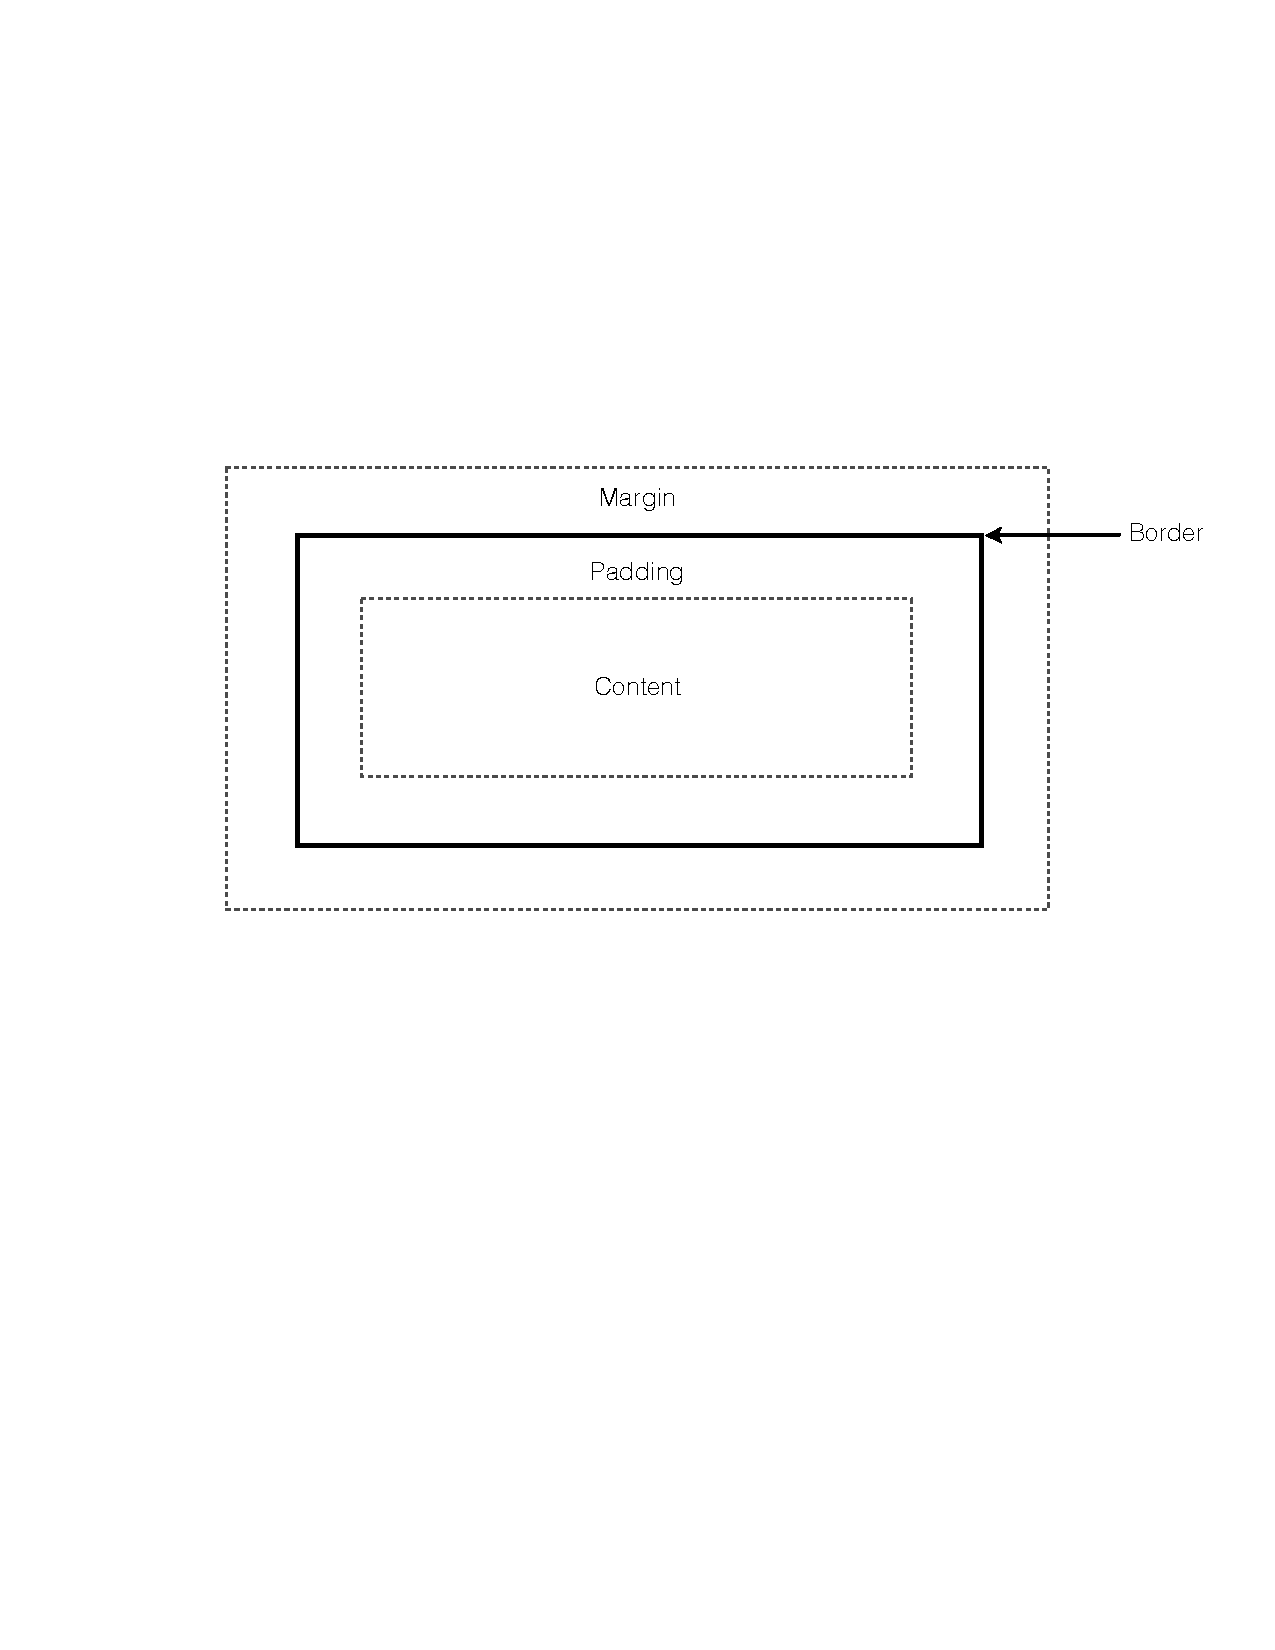
\includegraphics[width=\textwidth]{box_model}
	\caption{The Box Model}
	\label{fig:box_model}
\end{figure}

One should use \emph{margin} when spacing between elements is desired, and if one would like spacing from the content of the element to the border of the element, \emph{padding} should be used.





%----------------------------------------------------------------------------------------
%	CORE ELEMENTS
%----------------------------------------------------------------------------------------

\part{Core Elements}
%!TEX root = ../../main.tex

%!TEX root = ../../main.tex

\chapter{Icons}
\index{Icons}

Throughout the \giraf-software suite different icons will be used to reference different applications and functionalities. Refer to the sections below to see how and when to use these icons.

\section{\giraf Software Suite Icon}
\index{Icons}
The different applications in the \giraf software suite may want to refer to the software suite itself. To do this, the overall application icon seen in \figref{fig:overall_application_icon} can be used. This icon will also be used in some situations for indicating activity. \todo{Refer to a section describing activity indicators}

\begin{figure}[h]
	\centering
	
\includegraphics[scale=0.25]{placeholder}
	\caption{Overall application icon for the \giraf software suite}
	\label{fig:overall_application_icon}
\end{figure}

\section{Application-specific Icons}
\index{Icons}
Each application in the \giraf software suite must have its own icon. This icon should reflect the content and functionality of the application and must not be ambiguous. All application icons should furthermore use the icon-base seen in \figref{fig:application_specific_icon_base}. 
\\\\
Rendered icons must be available in sizes defined in the \href{http://developer.android.com/design/style/iconography.html}{Android Iconography article}. The foreground of the icon must be clear in any of these sizes. Furthermore, the icon must not appear smudged or otherwise distorted on any scale.

\begin{figure}[h]
	\centering
	
\includegraphics[width=0.15\textwidth]{application_specific_icon_base}
	\caption{Base for all application specific icon}
	\label{fig:application_specific_icon_base}
\end{figure}

\section{Icons used to represent functionality}
\index{Icons}
Specific icons may be used in buttons (See \texttt{GirafButton} in \gc) to represent functionality. The foreground of these icons must be gray-scaled and be quadratic (square). The functionality that the icon represents should be reflected in the icons itself. The icons should use the icon-base seen in \figref{fig:functionality_specific_icon_base}.

\begin{note}
	Please be aware that the actual icons should not be designed/rendered using the base as described above. Instead use the \texttt{GirafButton} from the \gc library. This will allow you to only design the actual foreground and not worry about the background (base).
\end{note}

\begin{figure}[h]
	\centering
	
\includegraphics[width=0.15\textwidth]{functionality_specific_icon_base}
	\caption{Base for all functionality-specific icons}
	\label{fig:functionality_specific_icon_base}
\end{figure}


%!TEX root = ../../main.tex

\chapter{Image Representation}
\index{Image}
\index{Pictogram}

For the following sections there exist a shared component called \androidinline{GirafPictogramItemView} which assists one to comply with the following design rules, for a guide on how to use this class see \appref{app:implementation_guide_for_pictures}.

\section{Appearance}
\label{sec:appearance}
In the \giraf software-suite there exist various types of images, such as pictograms and profile pictures. Images should be quadratic, have a white background (\colref{3.1}) regardless of content and have a black border (\colref{3.2}), as seen in \figref{fig:pictogram_image_view}. 

\begin{figure}[!htbp]
    \centering

    \begin{subfigure}[t]{0.4\textwidth}
    	\centering
        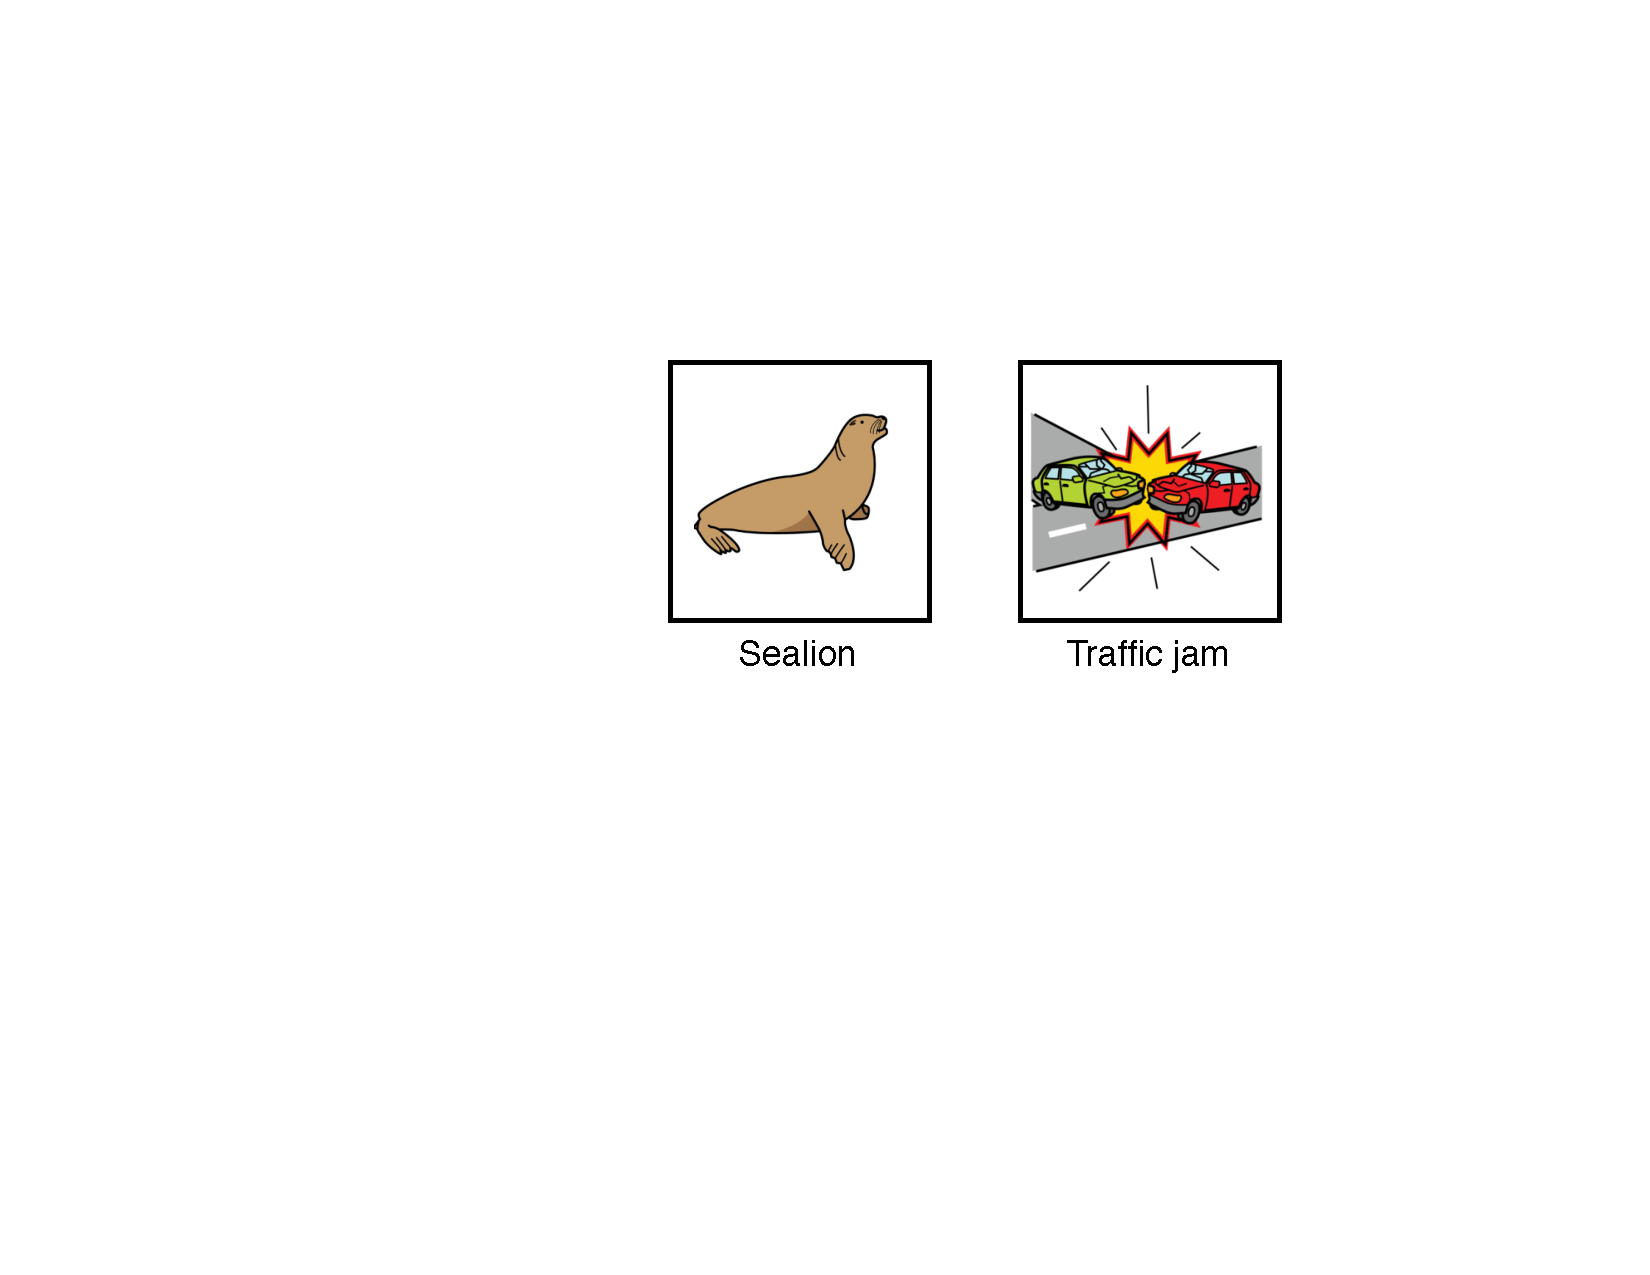
\includegraphics[scale=0.5]{pictogram_image_view_pictograms}
        \caption{Pictograms}
        \label{fig:pictogram_image_view_pictograms}
    \end{subfigure}
    \hspace{5em} 
    \begin{subfigure}[t]{0.4\textwidth}
    	\centering
        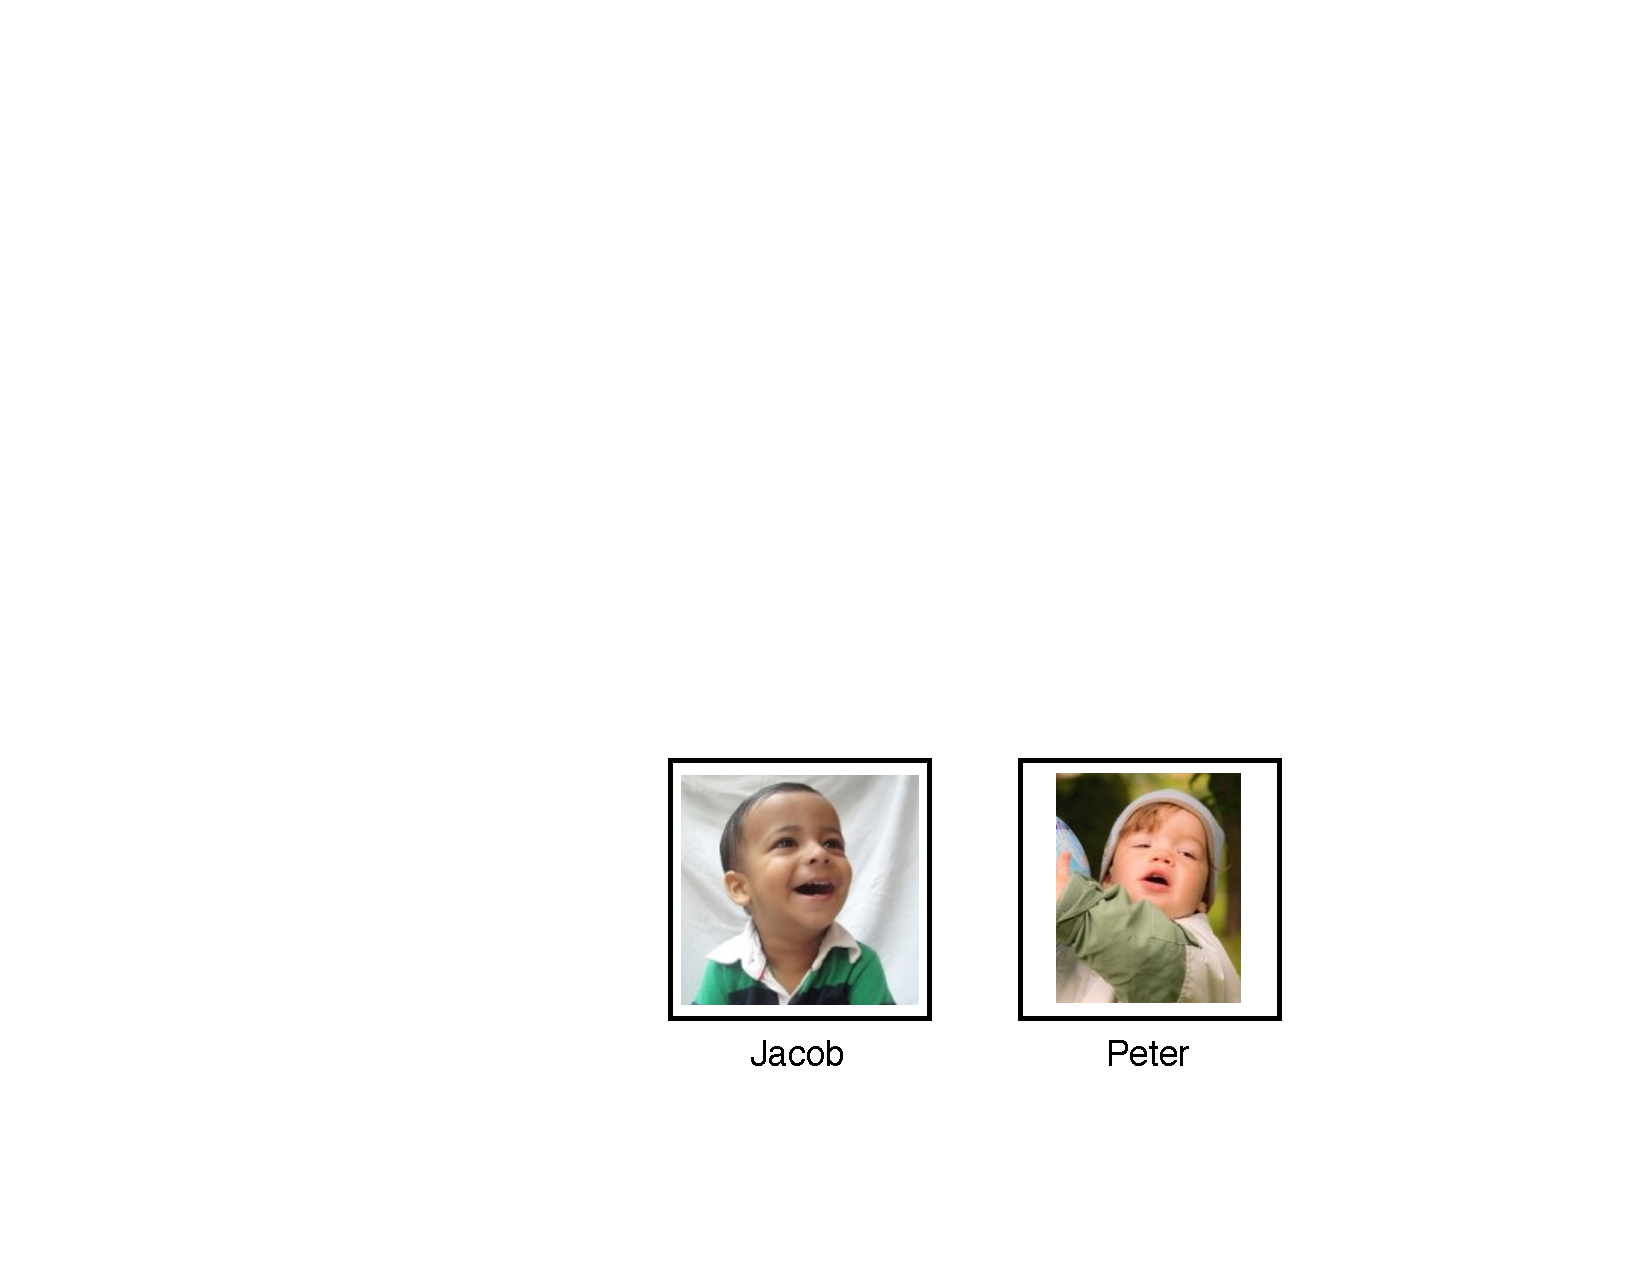
\includegraphics[scale=0.5]{pictogram_image_view_profiles}
        \caption{Profile pictures}
        \label{fig:pictogram_image_view_profiles}
    \end{subfigure}
    
    \caption{Image representation}
    \label{fig:pictogram_image_view}
\end{figure}

\begin{note}
	Profile pictures, as seen in \figref{fig:pictogram_image_view_profiles}, should, as the first profile (Jacob), fit to the canvas. However, many profile pictures are captured in a different way as seen in the second profile (Peter). It is wanted that in the future, when profile pictures are captured, that they only allow for pictures that have the layout of the first profile. For the sake of convenience and backwards compatibility we allow old profile pictures to be as the second.
\end{note}

\noindent
The image view should have a 10 dp padding so that the content gets spacing to the border as seen in \figref{fig:pictograms_padding}.

\begin{figure}[h]
	\centering
	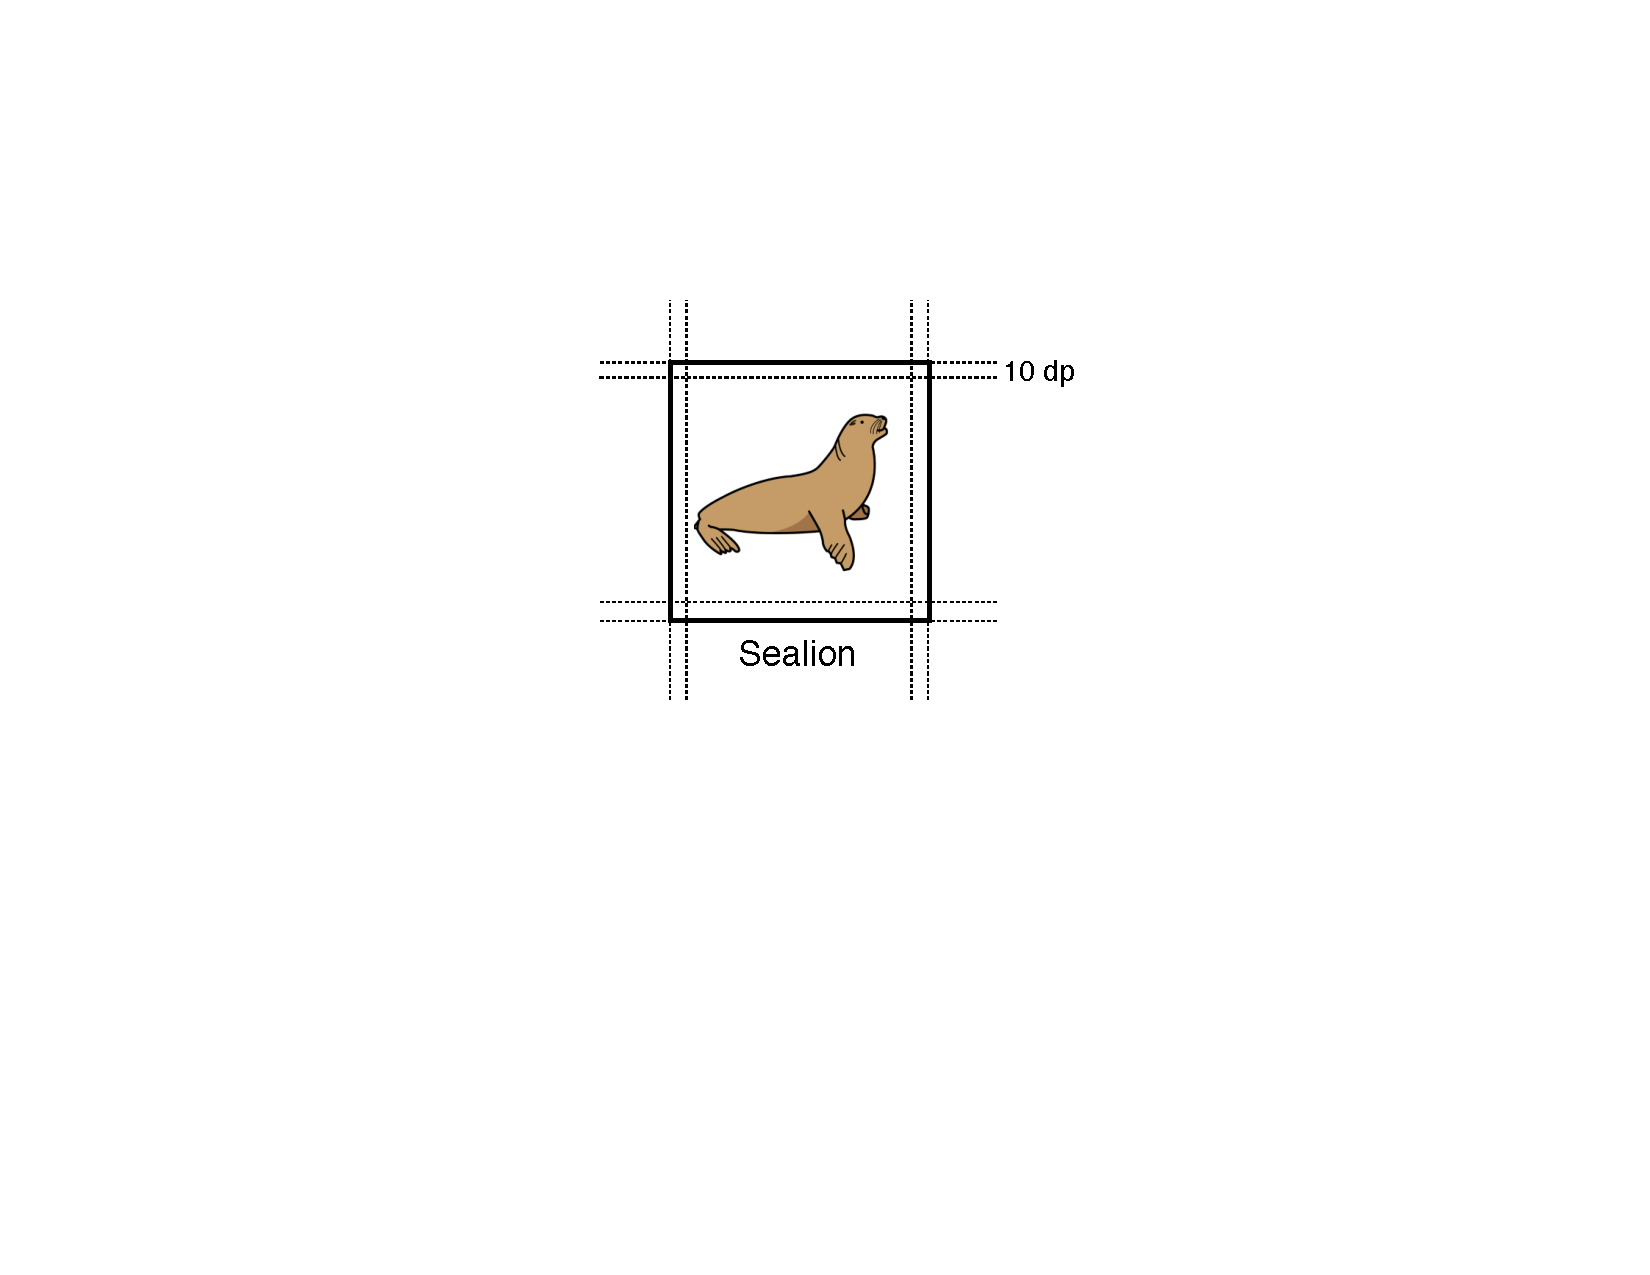
\includegraphics[width=0.35\textwidth]{pictograms_padding}
	\caption{Image representation}
	\label{fig:pictograms_padding}
\end{figure} 
\FloatBarrier

\subsection{Citizen view}
\label{sub:citizen_view}

When an image is present for a citizen it is not allowed for the image to be incomplete. See \figref{fig:citizen_image_view} for an example of how it should be shown to citizens and an example (\figref{fig:citizen_image_view_correct}) of how it should not be shown to citizens (\figref{fig:citizen_image_view_wrong}). 

\begin{figure}[!htbp]
    \centering

    \begin{subfigure}[t]{0.4\textwidth}
        \centering
        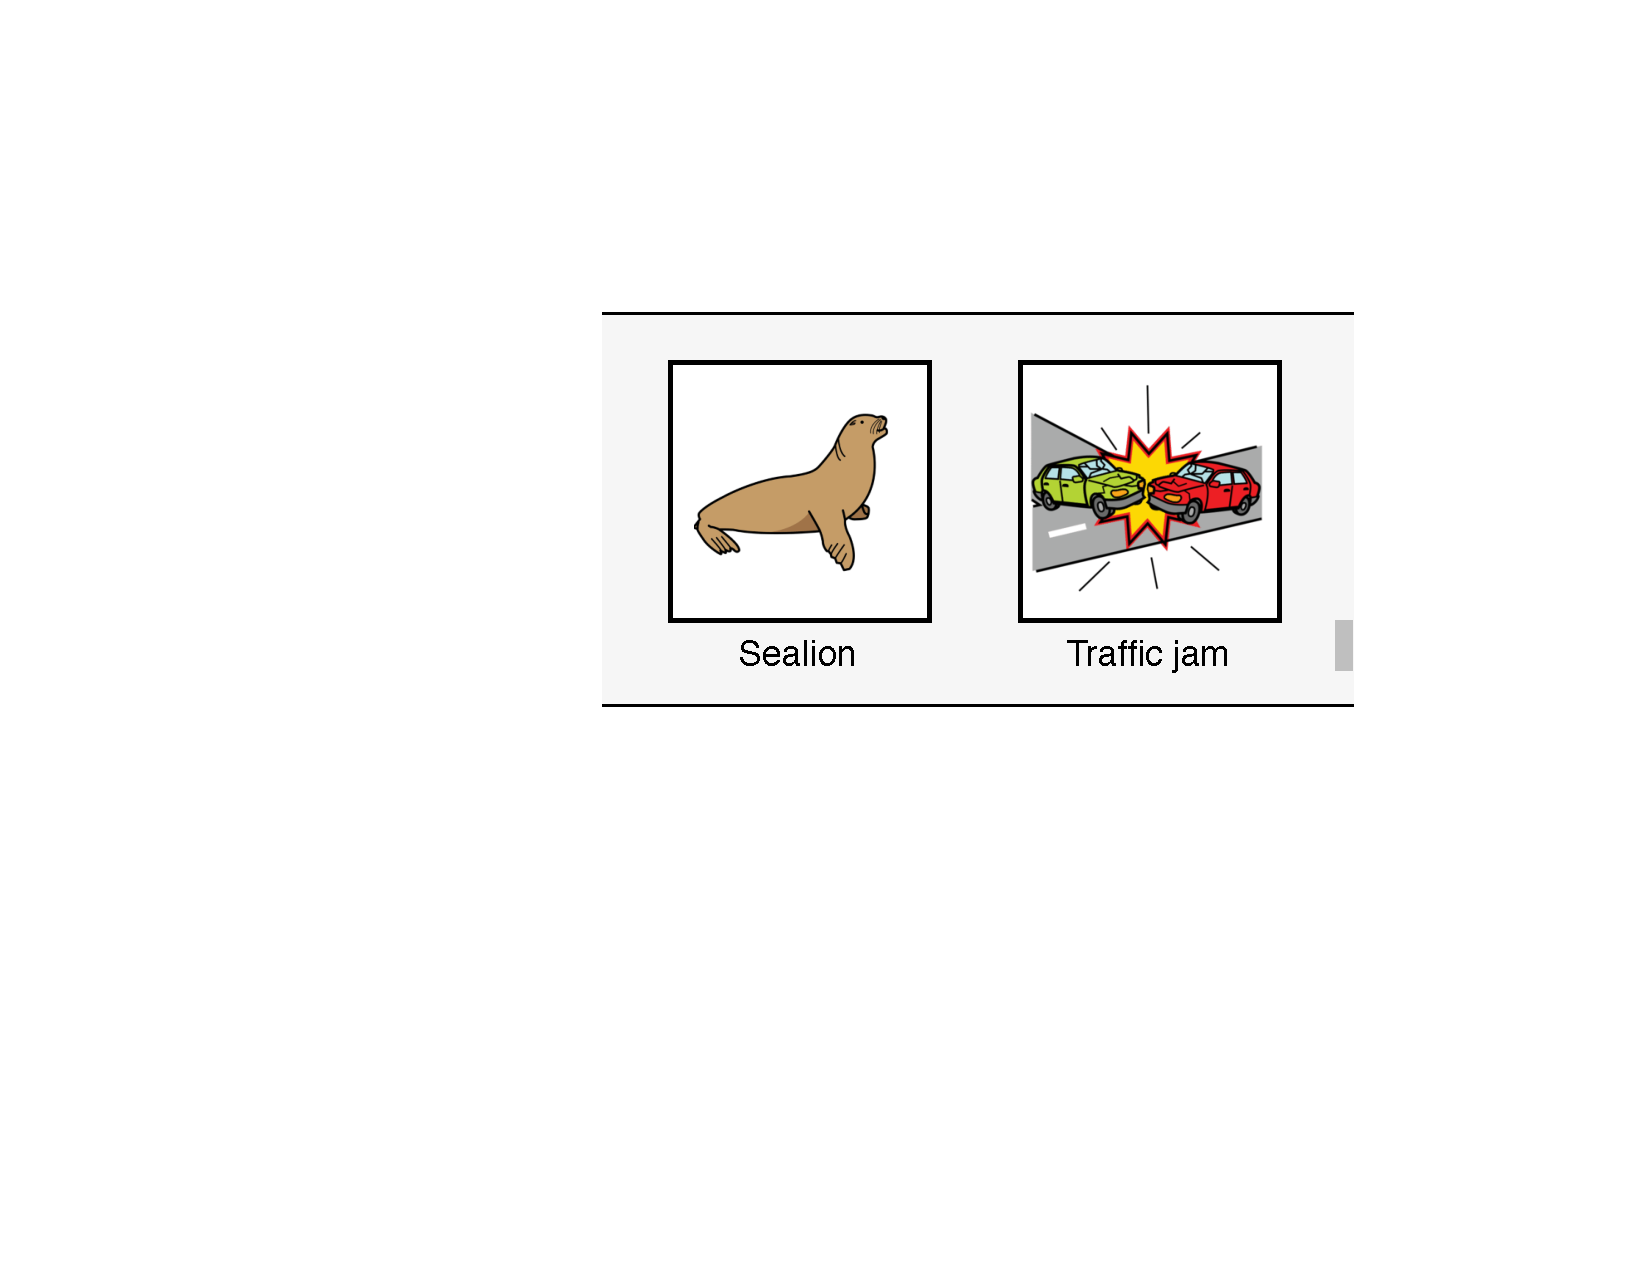
\includegraphics[scale=0.5]{citizen_view_correct}
        \caption{Correct citizen appearance}
        \label{fig:citizen_image_view_correct}
    \end{subfigure}
    \hspace{5em} 
    \begin{subfigure}[t]{0.4\textwidth}
        \centering
        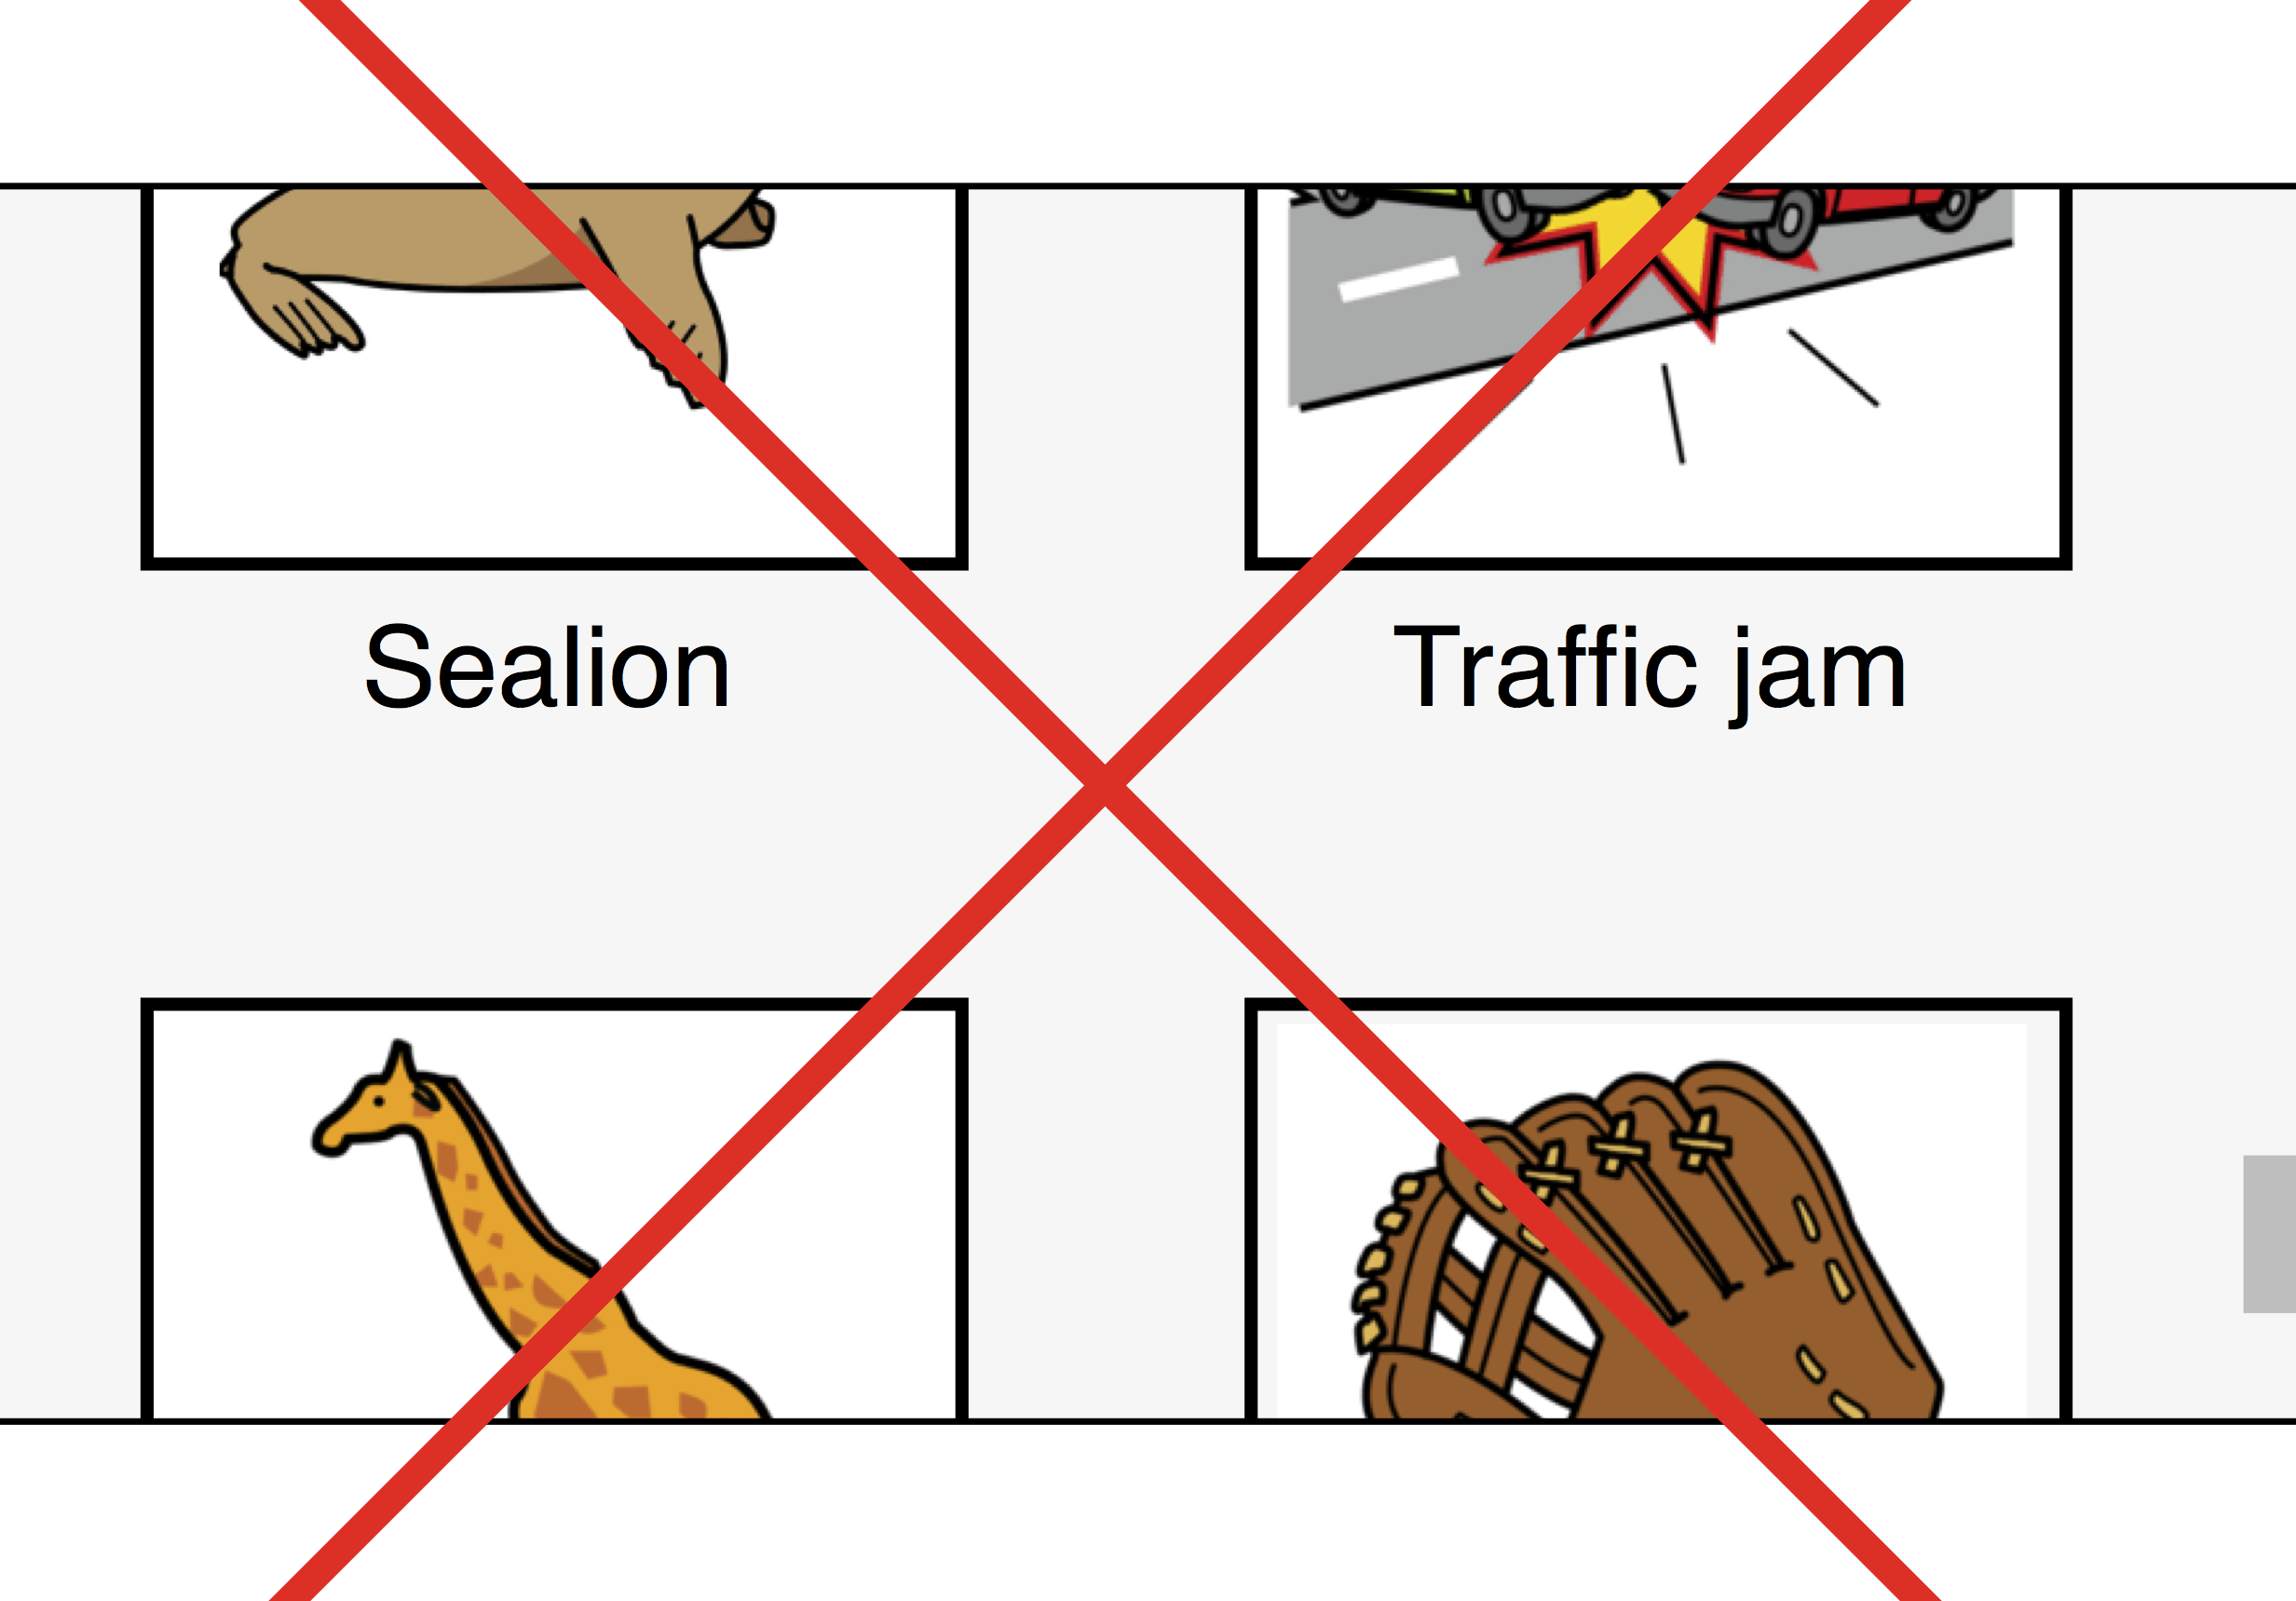
\includegraphics[scale=0.5]{citizen_view_wrong}
        \caption{Wrong citizen appearance}
        \label{fig:citizen_image_view_wrong}
    \end{subfigure}
    
    \caption{Citizen appearance explanation}
    \label{fig:citizen_image_view}
\end{figure}

\section{Marking}
\index{Marking}
\index{Selection}
\label{sec:marking}
It is often possible to mark images throughout the suite, and whenever this happens one should mark the background of the selected item with an orange color (\colref{3.3}), as seen in \figref{fig:pictograms_marked}. 

\begin{figure}[!htbp]
    \centering

    \begin{subfigure}[t]{0.4\textwidth}
    	\centering
        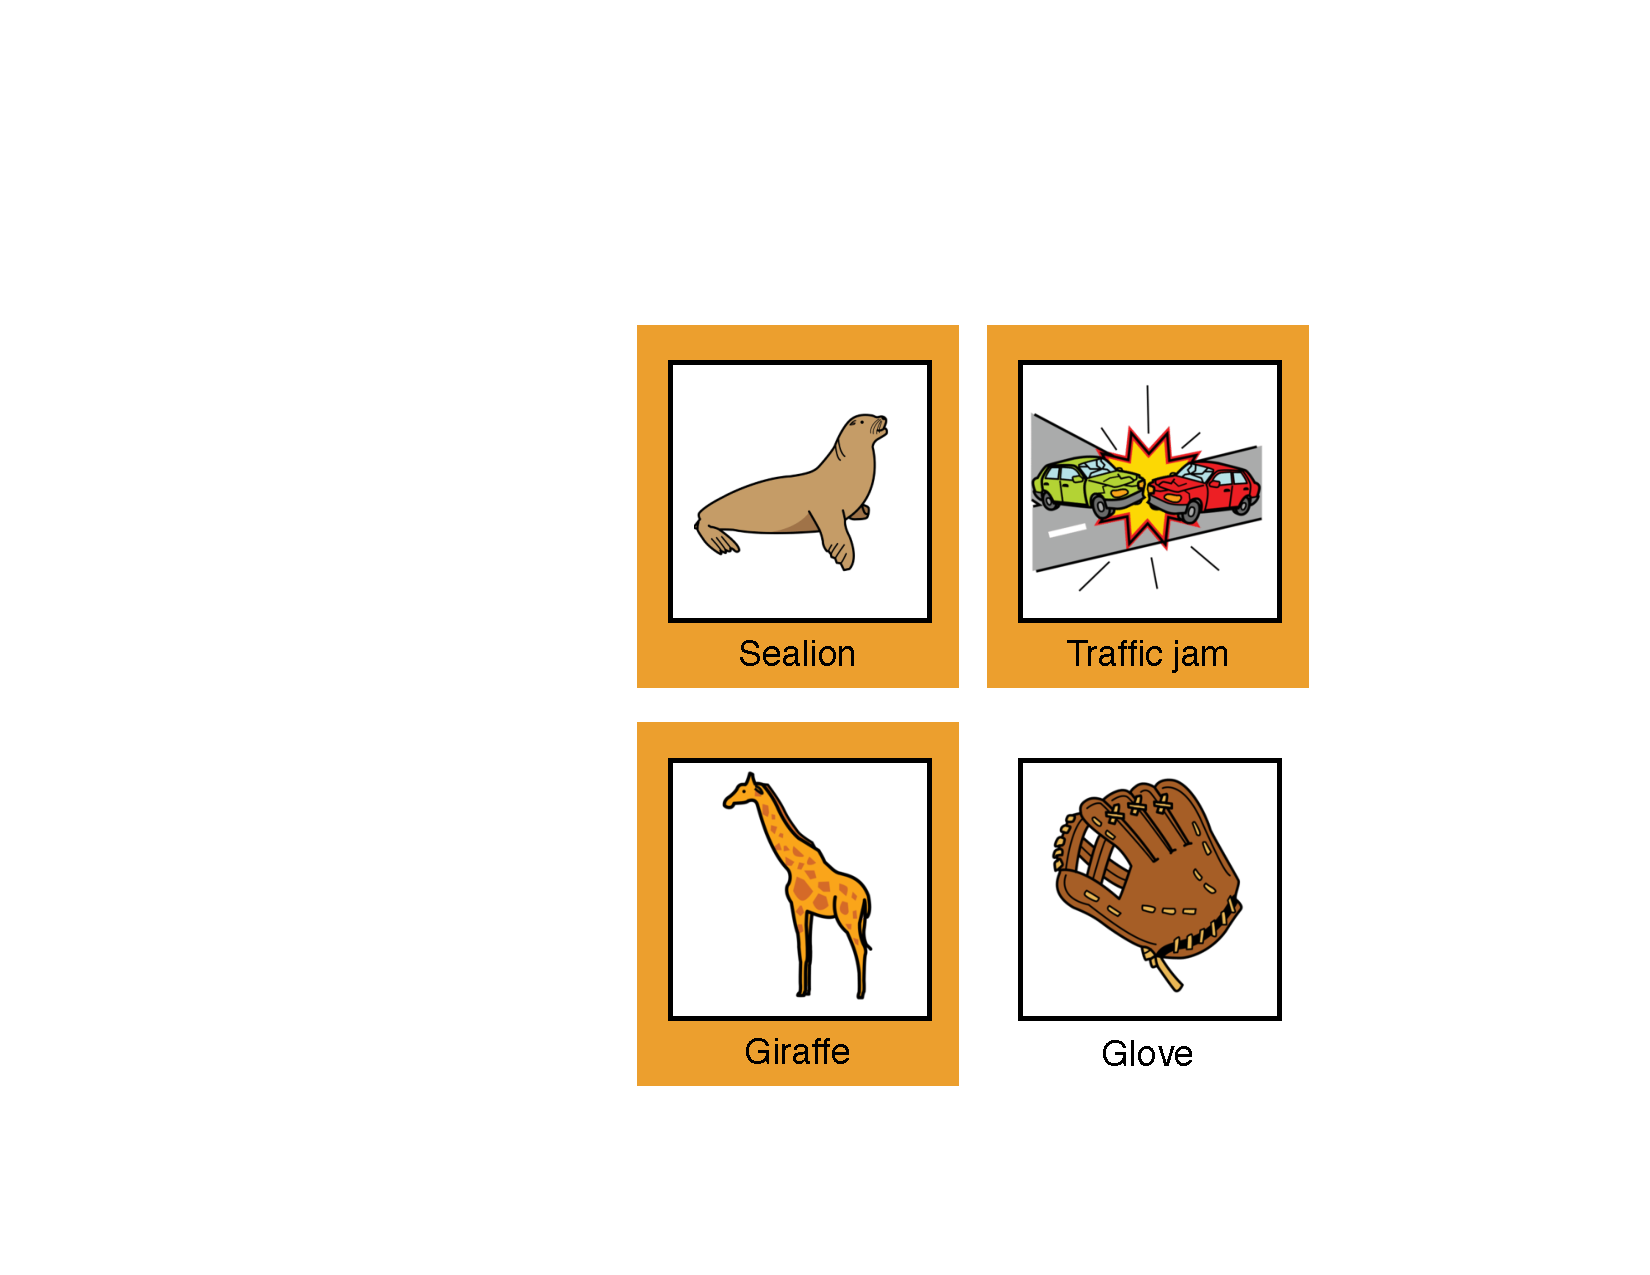
\includegraphics[scale=0.5]{pictograms_marked_correct}
        \caption{Corrected marking}
        \label{fig:pictograms_marked_corect}
    \end{subfigure}
    \hspace{5em} 
    \begin{subfigure}[t]{0.4\textwidth}
    	\centering
        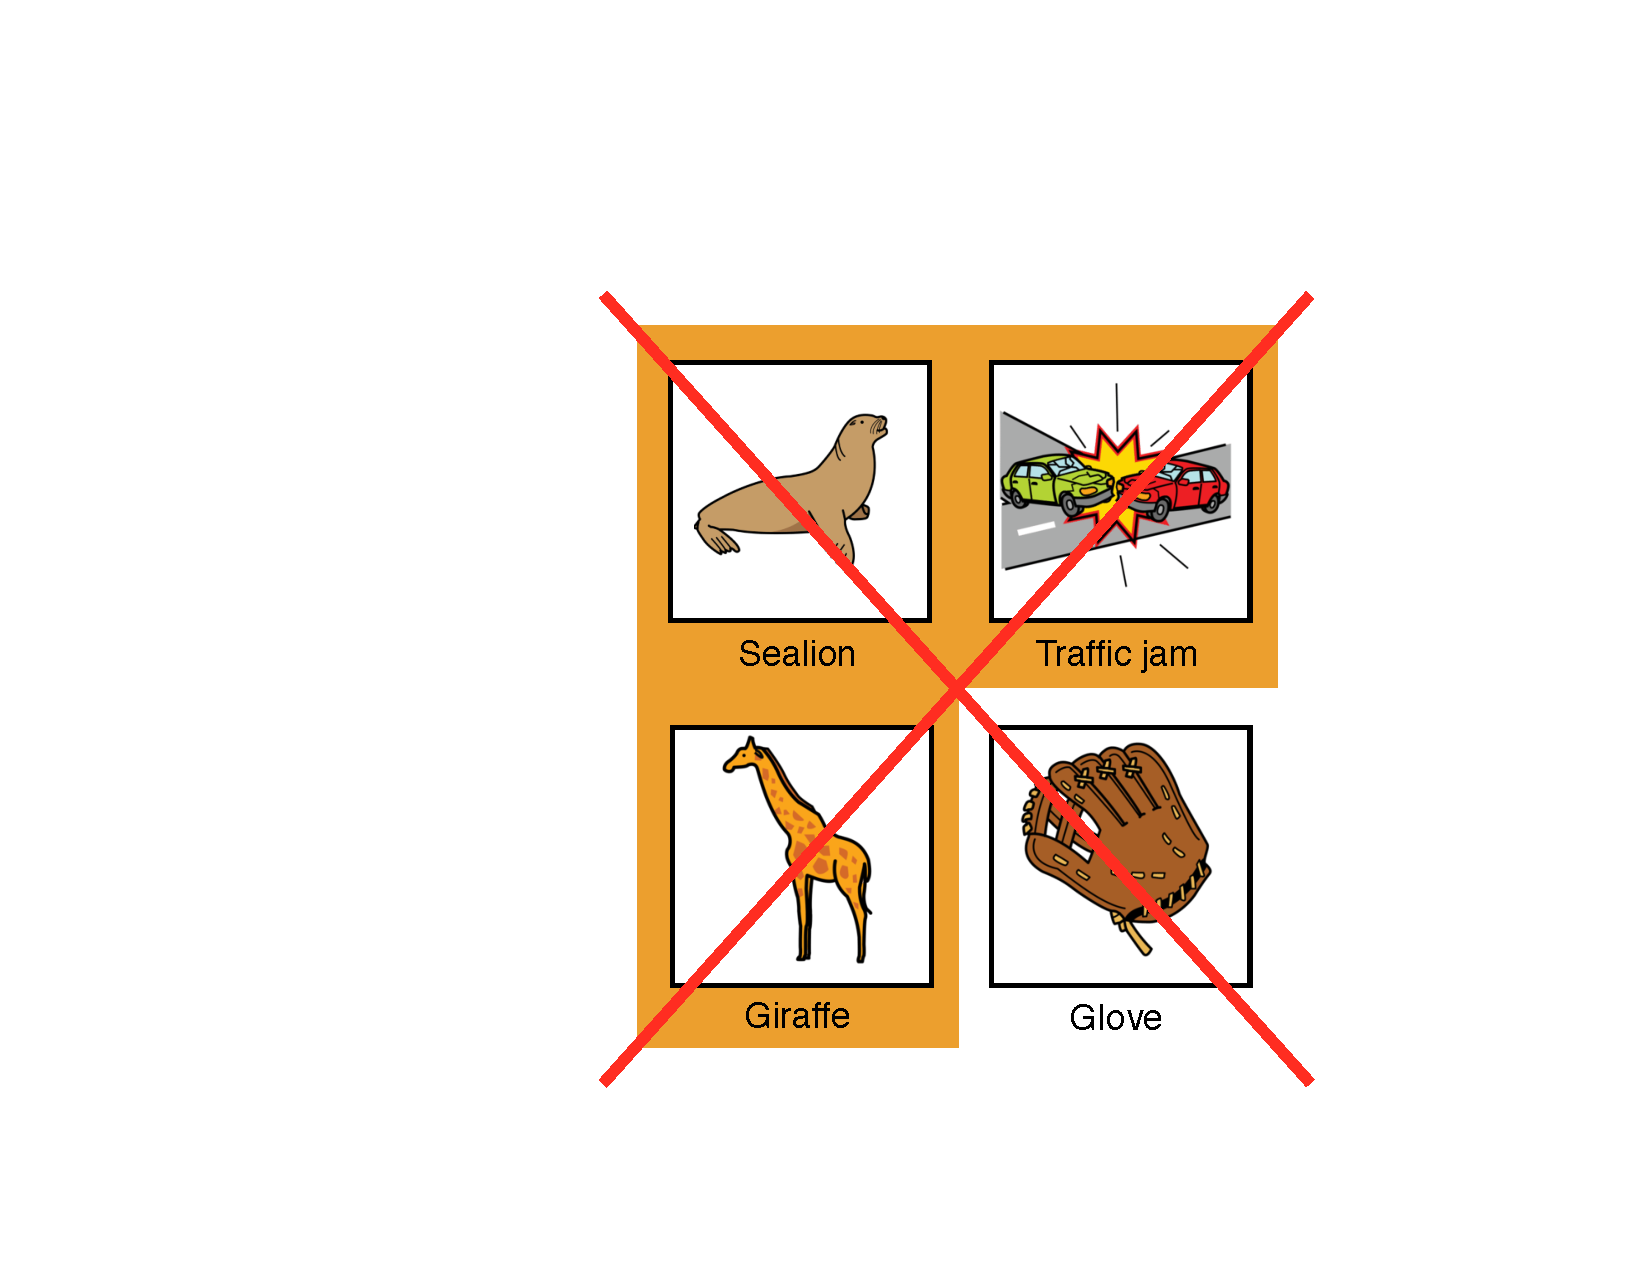
\includegraphics[scale=0.5]{pictograms_marked_wrong}
        \caption{Wrong marking}
        \label{fig:pictograms_marked_wrong}
    \end{subfigure}
    
    \caption{Marking of images}
    \label{fig:pictograms_marked}
\end{figure}

\begin{note}
	It is important that when having multiple marked images that there are some margin between these elements. This should be implemented as seen in \figref{fig:pictograms_marked_corect}, and not as seen in \figref{fig:pictograms_marked_wrong}.
\end{note} 

\section{Indicator overlay}
\index{Overlay}
\index{Overlay!Custom indicator}
\index{Overlay!Editable indicator}
\index{Indicator}
\index{Indicator!Editable indicator}
\index{Indicator!Custom indicator}
\index{Editable}
\label{sec:indicator_overlay}

If one wants to indicate that an image is editable, for instance when picking an icon for a category, the image should have an overlay indicating this as seen in \figref{fig:pictogram_indicator_overlay_editable}. Other types of indicators should look similar, e.g. when indicating that an image is a placeholder for a category it is indicated as seen in \figref{fig:pictogram_indicator_overlay_category}.

\begin{figure}[!htbp]
    \centering

    \begin{subfigure}[t]{0.4\textwidth}
        \centering
        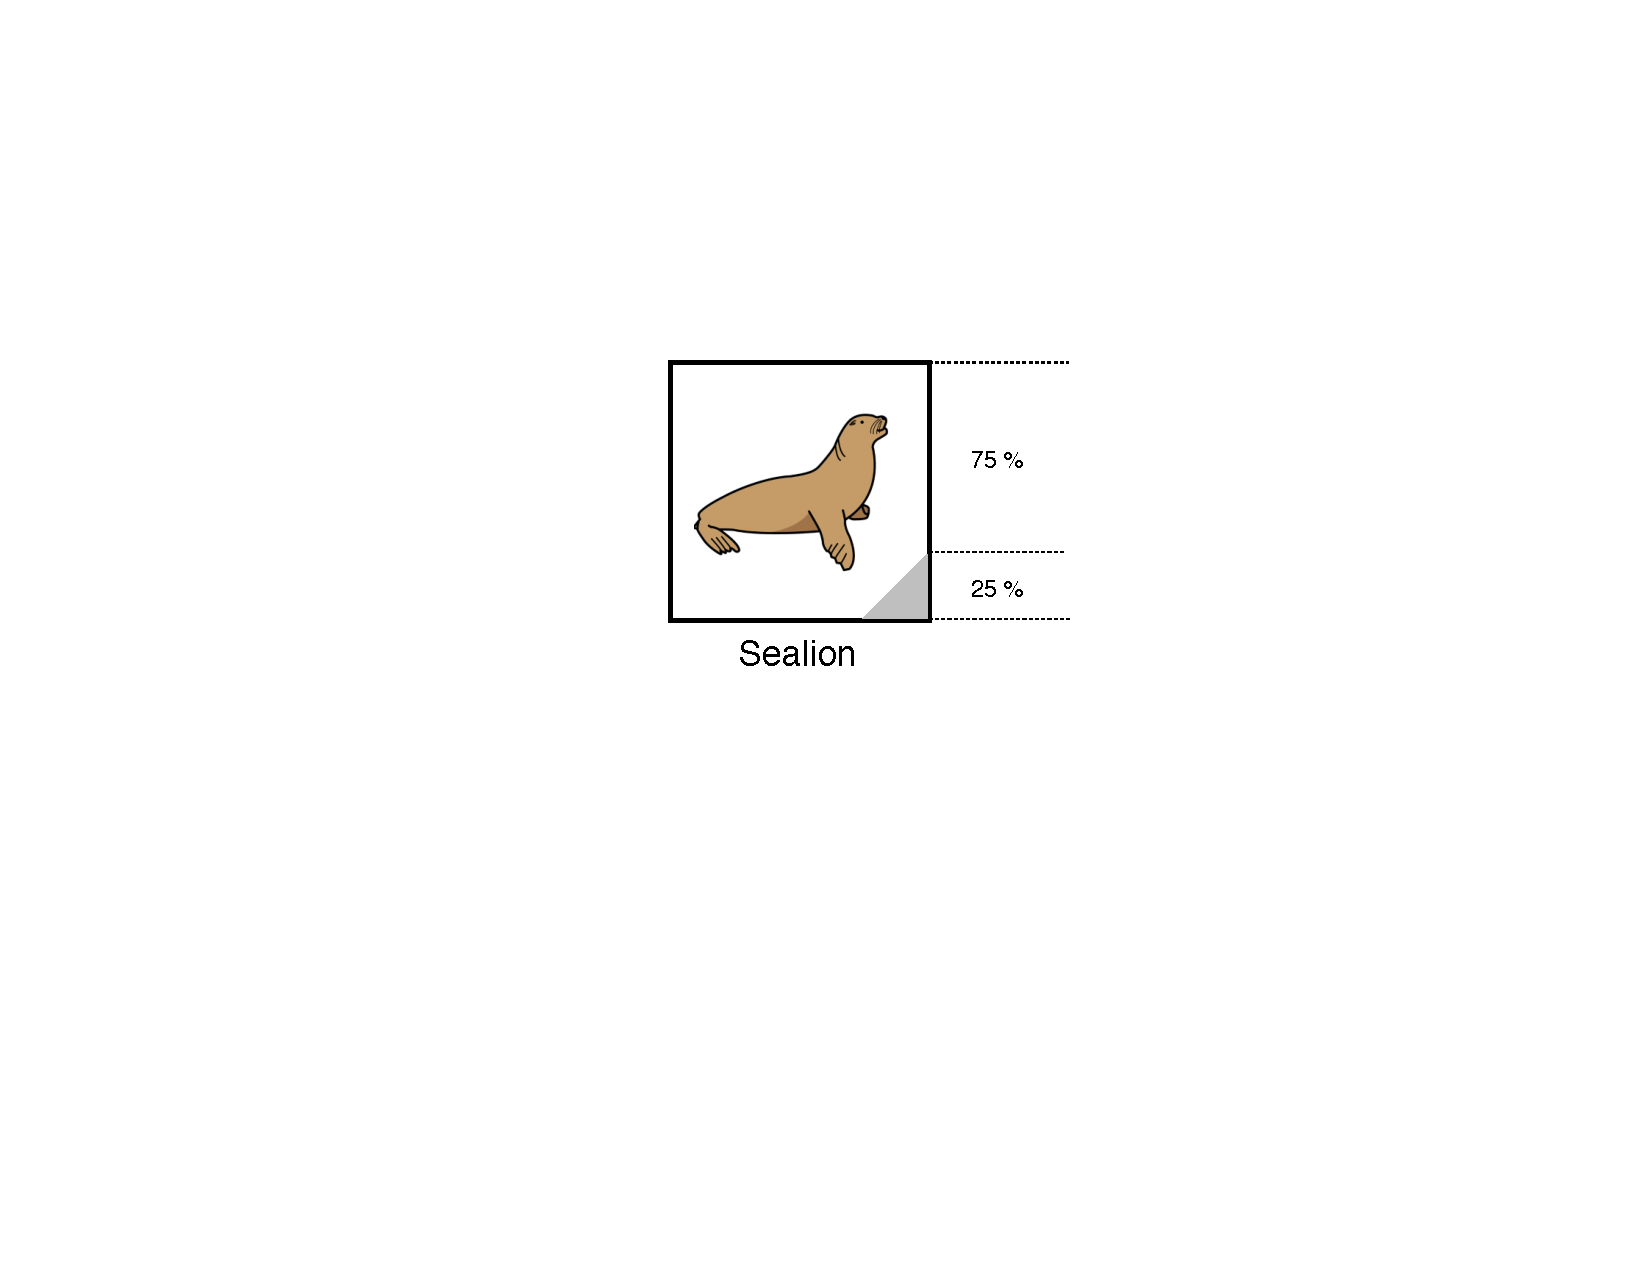
\includegraphics[scale=0.6]{pictogram_indicator_overlay_editable}
        \caption{Editable indicator}
        \label{fig:pictogram_indicator_overlay_editable}
    \end{subfigure}
    \hspace{5em} 
    \begin{subfigure}[t]{0.4\textwidth}
        \centering
        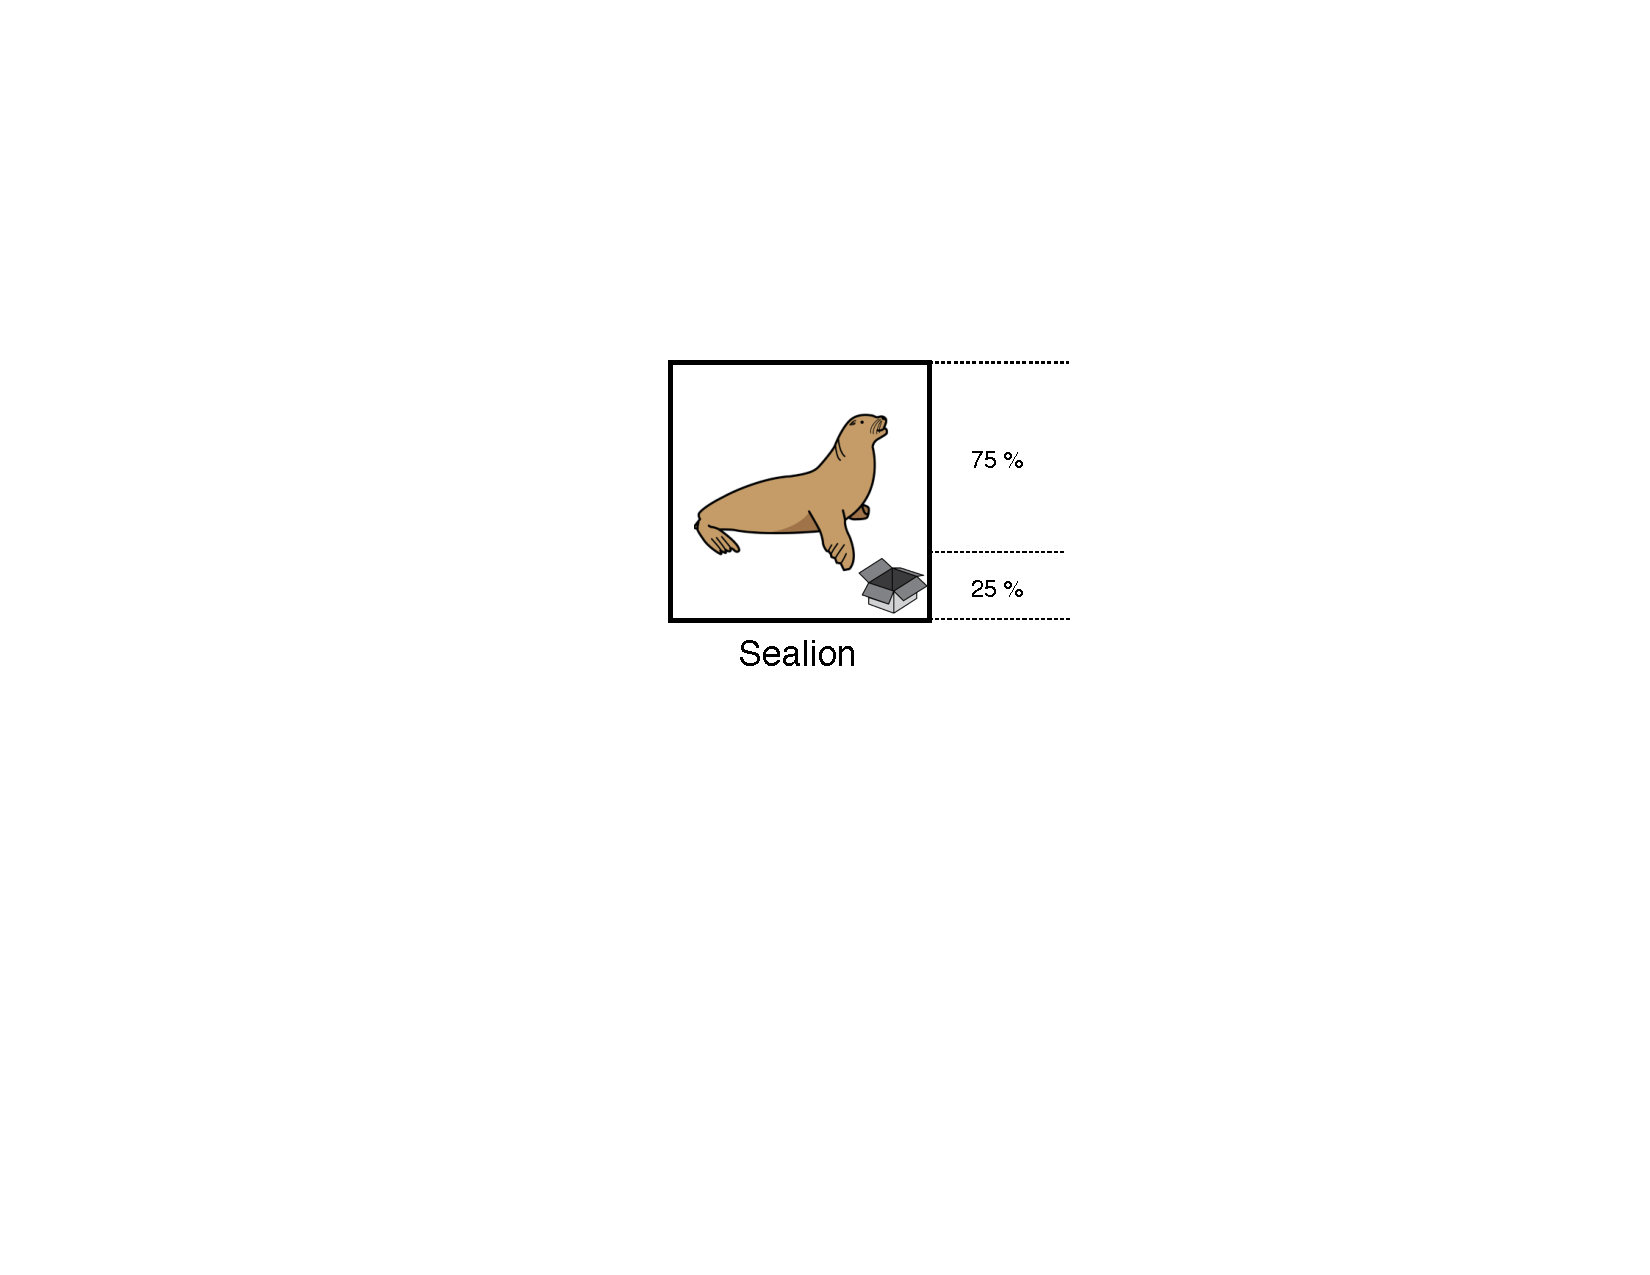
\includegraphics[scale=0.6]{pictogram_indicator_overlay_category}
        \caption{Category indicator}
        \label{fig:pictogram_indicator_overlay_category}
    \end{subfigure}
    
    \caption{Indicator overlays}
    \label{fig:pictograms_overlay}
\end{figure}


%!TEX root = ../../main.tex

\chapter{Typography}
% TODO: Write about the typography

\section{Fonts, Sizes and Colors}
When creating text fields in the \giraf software suite, is it imperative that they look alike across the entire suite. For this reason one should at all times use the default font-type in the applications. \\

\noindent The size of any text across the applications should always be given in ``SP'', and should always be readable on both 7 and 10 inch tablets. It is up to the developers of the individual applications to decide upon a specific text-size, but it should fit the general layout of the suite. \\

\noindent All text should by default be black (\#000000) across the suite when placed in buttons, views, etc. When creating hint text, e.g. when there are no applications present in the launcher, one should use the android implementation of Darker Gray\footnote{http://developer.android.com/reference/android/R.color.html\#darker\_gray}. When using the showcase library to highlight features, the text color of the help text should be white (\#FFFFFF), so it is readable on the dark background. 

%!TEX root = ../../main.tex

\chapter{Tone of Voice}
\index{Tone of voice}
\index{Voice}
When displaying messages to the user the following rules must be respected.

\section{Short and Precise}
All messages must be short and precise. If a part of a sentence is redundant, remove it. However, you must provide enough information to cover the whole situation.

\begin{exampleR}[Correct use]
	The application can only be started from a guardian profile
\end{exampleR}

\begin{exampleW}[Incorrect use]
	The application could not be started
\end{exampleW}

\begin{exampleW}[Incorrect use]
	The application could not be started unless you start it from a guardian profile. Please log onto a guardian profile to gain access to this application.
\end{exampleW}

\section{Addressing Users}
When referring to people with Autism Spectrum Disorder (ASD), use the word \textit{citizens}. When referring to either institutional- or legal guardians, use the word \textit{guardian}.

\begin{exampleR}[Correct use]
	The application cannot be started from a citizen-profile
\end{exampleR}

\begin{exampleW}[Incorrect use]
	The application cannot be started from a child-profile
\end{exampleW}

%!TEX root = ../../main.tex

\chapter{Application structure}
% TODO: Describe a generic application and how it should be structured. For instance the use of the topbar or sidemenu. Also talk about contextual menus.

\section{Top Bar}
\index{Action bar}
\index{Top bar}
An Android \androidinline{Activity} includes an optional top bar which if utilized should look like \figref{fig:top_bar_example}. A top bar should have the standard top bar size in Android.\\
The top bar should only include buttons related to the entire Activity and should not depend on the context inside the activity.

\begin{note}
Such a top bar is easily achieved by letting your \androidinline{Activity} extend the \androidinline{GirafActivity} from the Giraf Components library.
\end{note}

\begin{figure}[!htbp]
        \centering
        
\includegraphics[width=0.75\textwidth]{pictures/application_structure/topbar}
        \caption{Top bar example}
        \label{fig:top_bar_example}
\end{figure}

\FloatBarrier


\section{Side Bar}
\index{Side bar}

Side bars need not, but may be contextual. It is recommended to use side bars to switch between content of applications. A side bar should look like \figref{fig:side_bar_example}.

\begin{figure}[!htbp]
        \centering
        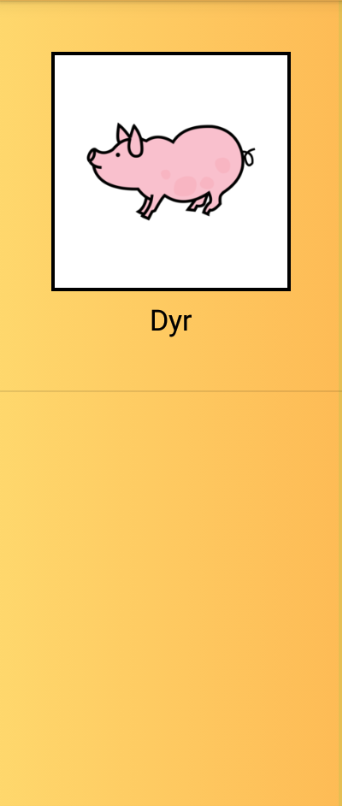
\includegraphics[width=0.25\textwidth]{pictures/application_structure/sidebar}
        \caption{Side bar example}
        \label{fig:side_bar_example}
\end{figure}

\FloatBarrier


\section{Bottom bar}
\index{Bottom bar}
Bottom bars should be entirely contextual and depend on the current content displayed in the current \androidinline{Activity}. A bottom bar should look like \figref{fig:bottom_bar_example}.

\begin{figure}[!htbp]
        \centering
        
\includegraphics[width=0.75\textwidth]{pictures/application_structure/bottombar}
        \caption{Bottom bar example}
        \label{fig:bottom_bar_example}
\end{figure}

\FloatBarrier


\section{Content}
The main content of applications should be in the center of the layout and any menu bars should be above, under, and to the sides of the main content. 

\begin{note}
We recommend using Android \androidinline{Fragment} instances to manage content of an \androidinline{Activity} if the main content of an Android \androidinline{Activity} needs to change between different content that needs to be controlled differently. 
\end{note}


\section{Clickable Elements}
All elements that are clickable must have a safety-distance to other elements. This will ensure that the user does not accidentally press the wrong thing and ultimately does something wrong. This safety distance may be achieved using several different methods. Please refer to the following sections. \figref{fig:correct_element_spacing} shows an example of correct item spacing while \figref{fig:incorrect_element_spacing} shows an example of incorrect item spacing.
\\\\
Elements must have a safety distance to \ldots
\index{Margin}
\begin{itemize}
        \item Other clickable elements
        \item Borders of it's container
        \item Borders of the tablet
\end{itemize}

\begin{figure}[!htbp]
    \centering
    \begin{subfigure}[t]{0.4\textwidth}
        \centering
        
\includegraphics[scale=0.1]{correct_element_spacing}
        \caption{Correct item spacing}
        \label{fig:correct_element_spacing}
    \end{subfigure}
    \hspace{5em} 
    \begin{subfigure}[t]{0.4\textwidth}
        \centering
        
\includegraphics[scale=0.1]{incorrect_element_spacing}
        \caption{Incorrect item spacing}
        \label{fig:incorrect_element_spacing}
    \end{subfigure}
    
    \caption{Examples of correct and incorrect element spacing}
    \label{fig:element_spacing_examples}
\end{figure}

\subsection{Element Margin}
\index{Margin}
Elements may be spaced apart from each other using margin on the individual elements. The distance between the elements should be consistent throughout all activities of any given application. \figref{fig:element_margin_example} shows an example of the margin for a given element.. 

\begin{figure}[h]
        \centering
        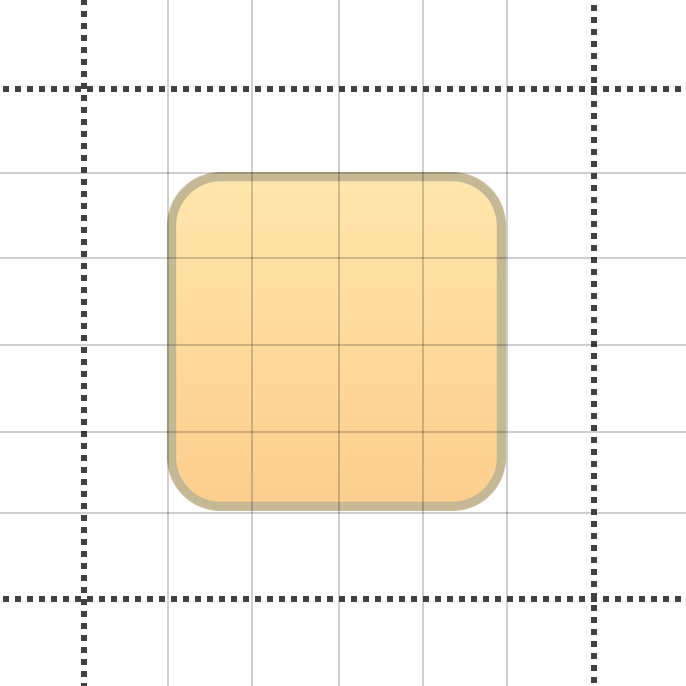
\includegraphics[width=0.25\textwidth]{element_margin_example}
        \caption{Example of element margin}
        \label{fig:element_margin_example}
\end{figure}

\begin{note}
        If margin is used inside a container each element with margin will also be a certain distance from the borders of that specific container. If, for instance, an element has a margin of $10$, then this element would be a distance of $10$ from the borders of the container. This means that there \textit{might} not be need for any padding on the given container.
\end{note}

\subsubsection{Consistent Margin}
\index{Margin}
Elements of the same type appearing in the same context must have the same distance to other elements. However, if the elements appear in an order, for example a horizontal list, the first and last element may differ. For instance, the first element may have a smaller left-margin and the last element may have a smaller right-margin. \figref{fig:element_margin_consistency} shows an illustration of this example.

\begin{figure}[h]
        \centering
        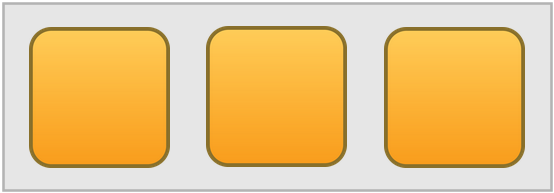
\includegraphics[width=0.45\textwidth]{element_margin_consistency}
        \caption{Example of element margin}
        \label{fig:element_margin_consistency}
\end{figure}


\subsection{Container Padding}
\index{Padding}
Each container should provide some padding for its content. This padding should be somewhat identical to the spacing between elements inside the container. \figref{fig:container_padding_example} shows an example of a container with padding. 

\begin{figure}[h]
        \centering
        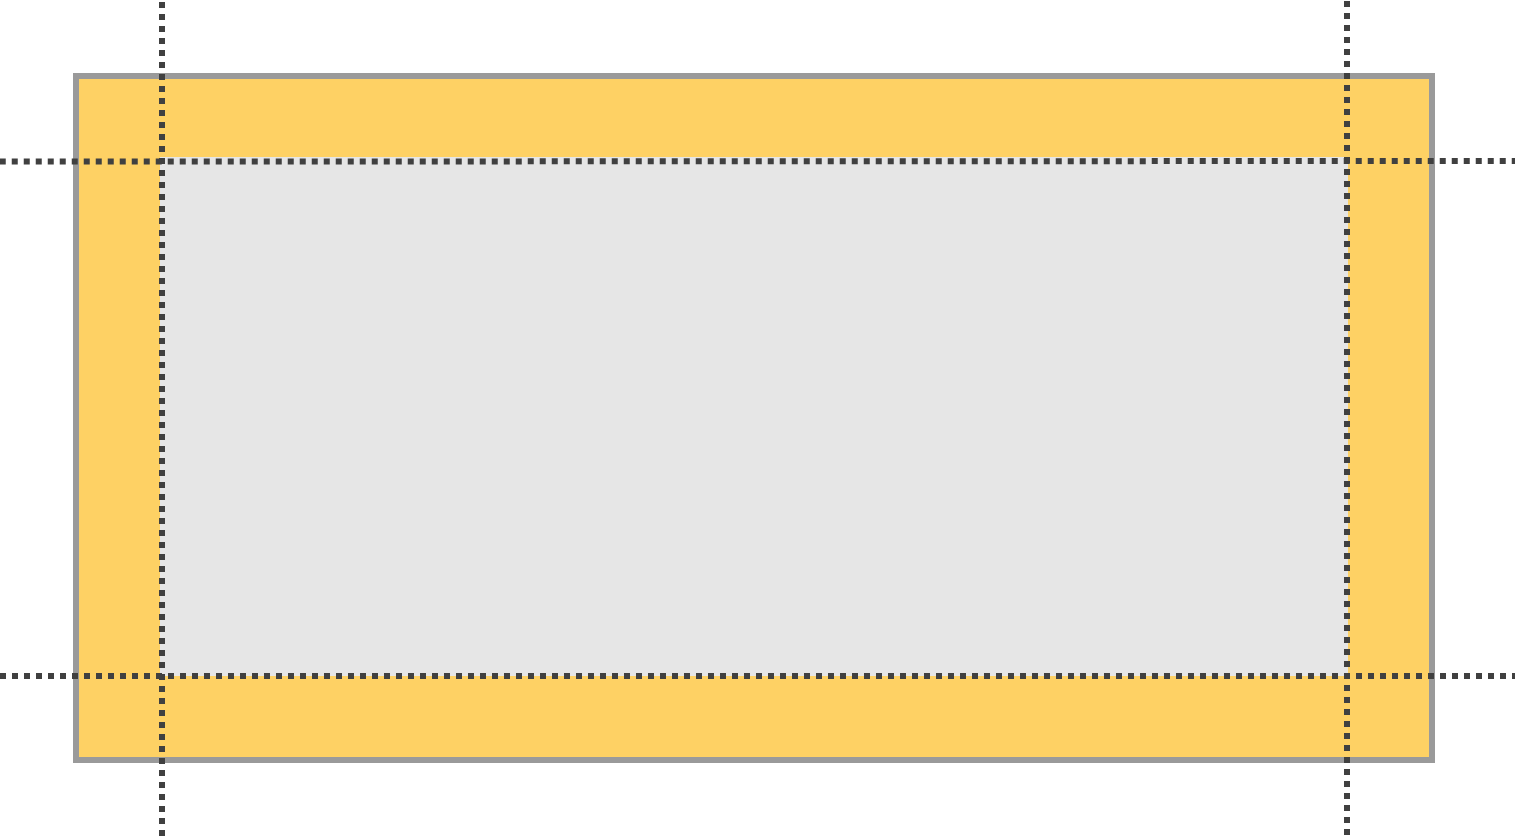
\includegraphics[width=0.65\textwidth]{container_padding_example}
        \caption{Example of a container with padding}
        \label{fig:container_padding_example}
\end{figure}

\begin{note}
        Whenever the content of the container can be scrolled through (for example a \texttt{GridView}) a property called \texttt{clipToPadding} must be set to \texttt{false}. Please refer to the \href{http://developer.android.com/reference/android/view/ViewGroup.html#attr_android:clipToPadding}{Android documentation} for additional information.
\end{note}\todo{The effect of this could be explained more clearly using a figure}


%!TEX root = ../../main.tex

\chapter{Colors}
\index{Colors}
Throughout this chapter a single color in each entry will denote a solid color, while two colors in an entry will denote a gradient between the two colors.

\section{Text and Background}
\index{Colors!Text color}
\index{Colors!Background color}
These colors should be used throughout any application.

\begin{table}[!htbp]
	\begin{tabularx}{\textwidth}{c X r c}
		\collabel{1.1}
		& Regular text-color 
		& \texttt{\#000000} & \cellcolor[HTML]{000000}\phantom{--} \\ \hline
	\end{tabularx}
\end{table}

\begin{table}[!htbp]
	\begin{tabularx}{\textwidth}{c X r c}
		\collabel{1.2}
		& Text-color used to indicate placeholder or hint-texts 
		& \texttt{\#AAAAAA} & \cellcolor[HTML]{AAAAAA}\phantom{--} \\ \hline
	\end{tabularx}
\end{table}

\begin{table}[!htbp]
	\begin{tabularx}{\textwidth}{c X r c}
		\collabel{1.3}
		& Background-color for any applications window background 
		& \texttt{\#000000} & \cellcolor[HTML]{000000}\phantom{--} \\ \hline
	\end{tabularx}
\end{table}

\begin{table}[!htbp]
	\begin{tabularx}{\textwidth}{c X r c}
		\collabel{1.4}
		& Background-color for any activity 
		& \texttt{\#E9E9E9} & \cellcolor[HTML]{E9E9E9}\phantom{--} \\ \hline
	\end{tabularx}
\end{table}

\section{Buttons}
\index{Colors!Button colors}
All buttons in the \giraf software suite should use these colors for buttons. Please note that all gradients defined below are from top to bottom. Also note that the colors for the disabled button must be slightly transparent ($65\%$).

\begin{table}[!htbp]
	\begin{tabularx}{\textwidth}{c X r c r c}
		\collabel{2.1}
		& Regular button background 
		& \texttt{\#FFCD59} & \cellcolor[HTML]{FFCD59}\phantom{--}
		& \texttt{\#FF9D00} & \cellcolor[HTML]{FF9D00}\phantom{--} \\ \hline
	\end{tabularx}
\end{table}

\begin{table}[!htbp]
	\begin{tabularx}{\textwidth}{c X r c r c}
		\collabel{2.2}
		& Regular button stroke/border 
		& ~ & ~
		& \texttt{\#8A6E00} & \cellcolor[HTML]{8A6E00}\phantom{--} \\ \hline
	\end{tabularx}
\end{table}

\begin{table}[!htbp]
	\begin{tabularx}{\textwidth}{c X r c r c}
		\collabel{2.2}
		& Pressed button background 
		& \texttt{\#D4AD2F} & \cellcolor[HTML]{D4AD2F}\phantom{--}
		& \texttt{\#FF9D00} & \cellcolor[HTML]{FF9D00}\phantom{--} \\ \hline
	\end{tabularx}
\end{table}

\begin{table}[!htbp]
	\begin{tabularx}{\textwidth}{c X r c r c}
		\collabel{2.3}
		Pressed button stroke/border 
		& ~ & ~
		& \texttt{\#493700} & \cellcolor[HTML]{493700}\phantom{--} \\ \hline
	\end{tabularx}
\end{table}

\begin{table}[!htbp]
	\begin{tabularx}{\textwidth}{c X r c r c}
		\collabel{2.4}
		& Focused button background 
		& \texttt{\#FF9D00} & \cellcolor[HTML]{FF9D00}\phantom{--}
		& \texttt{\#FF5900} & \cellcolor[HTML]{FF5900}\phantom{--} \\ \hline
	\end{tabularx}
\end{table}

\begin{table}[!htbp]
	\begin{tabularx}{\textwidth}{c X r c r c}
		\collabel{2.5}
		& Focused button stroke/border 
		& ~ & ~
		& \texttt{\#8A6E00} & \cellcolor[HTML]{8A6E00}\phantom{--} \\ \hline
	\end{tabularx}
\end{table}

\begin{table}[!htbp]
	\begin{tabularx}{\textwidth}{c X r c r c}
		\collabel{2.6}
		& Focused button background 
		& \texttt{\#FAD355} & \cellcolor[HTML]{FAD355}\phantom{--}
		& \texttt{\#FEBE40} & \cellcolor[HTML]{FEBE40}\phantom{--} \\ \hline
	\end{tabularx}
\end{table}

\begin{table}[!htbp]
	\begin{tabularx}{\textwidth}{c X r c r c}
		\collabel{2.7}
		& Focused button stroke/border 
		& ~ & ~
		& \texttt{\#E4AE4E} & \cellcolor[HTML]{E4AE4E}\phantom{--} \\ \hline
	\end{tabularx}
\end{table}

\section{Images}
\index{Image}
\index{Colors!Image}

\begin{table}[!htbp]
	\begin{tabularx}{\textwidth}{c X r c}
		\collabel{3.1}
		& Image background-color
		& \texttt{\#FFFFFF} & \cellcolor[HTML]{FFFFFF}\phantom{--} \\ \hline
	\end{tabularx}
\end{table}

\begin{table}[!htbp]
	\begin{tabularx}{\textwidth}{c X r c}
		\collabel{3.2}
		& Image border-color
		& \texttt{\#000000} & \cellcolor[HTML]{000000}\phantom{--} \\ \hline
	\end{tabularx}
\end{table}

\begin{table}[!htbp]
	\begin{tabularx}{\textwidth}{c X r c}
		\collabel{3.3}
		& Image marking-color
		& \texttt{\#FED76C} & \cellcolor[HTML]{FED76C}\phantom{--} \\ \hline
	\end{tabularx}
\end{table}

\section{Action Bar}
\index{Action bar}
\index{Colors!Action bar}
All applications that use action bars must use the following colors. Please notice that the gradient for the topbar is from top to bottom.

\begin{table}[!htbp]
	\begin{tabularx}{\textwidth}{c X r c r c}
		\collabel{4.1}
		& Background of any action bar
		& \texttt{\#FDBB55} & \cellcolor[HTML]{FDBB55}\phantom{--}
		& \texttt{\#FED76C} & \cellcolor[HTML]{FED76C}\phantom{--} \\ \hline
	\end{tabularx}
\end{table}

\begin{table}[!htbp]
	\begin{tabularx}{\textwidth}{c X r c r c}
		\collabel{4.2}
		& Stroke/border of the action bar 
		& ~ & ~
		& \texttt{\#E5BE53} & \cellcolor[HTML]{E5BE53}\phantom{--} \\ \hline
	\end{tabularx}
\end{table}


\section{Week indicators}
\index{Week indicators}
\index{Colors!Week indicators}
These colors must be used whenever a certain weekday is referenced. Note that colors are primarily used to increase the usability for citizens.


\begin{table}[!htbp]
	\begin{tabularx}{\textwidth}{c X r c r c}
		\collabel{5.1}
		& Monday 
		& ~ & ~
		& \texttt{\#007700} & \cellcolor[HTML]{007700}\phantom{--} \\ \hline
	\end{tabularx}
\end{table}

\begin{table}[!htbp]
	\begin{tabularx}{\textwidth}{c X r c r c}
		\collabel{5.2}
		& Tuesday 
		& ~ & ~
		& \texttt{\#800080} & \cellcolor[HTML]{800080}\phantom{--} \\ \hline
	\end{tabularx}
\end{table}

\begin{table}[!htbp]
	\begin{tabularx}{\textwidth}{c X r c r c}
		\collabel{5.3}
		& Wednesday 
		& ~ & ~
		& \texttt{\#FF8500} & \cellcolor[HTML]{FF8500}\phantom{--} \\ \hline
	\end{tabularx}
\end{table}

\begin{table}[!htbp]
	\begin{tabularx}{\textwidth}{c X r c r c}
		\collabel{5.4}
		& Thursday 
		& ~ & ~
		& \texttt{\#0000FF} & \cellcolor[HTML]{0000FF}\phantom{--} \\ \hline
	\end{tabularx}
\end{table}

\begin{table}[!htbp]
	\begin{tabularx}{\textwidth}{c X r c r c}
		\collabel{5.5}
		& Friday 
		& ~ & ~
		& \texttt{\#FFDD00} & \cellcolor[HTML]{FFDD00}\phantom{--} \\ \hline
	\end{tabularx}
\end{table}

\begin{table}[!htbp]
	\begin{tabularx}{\textwidth}{c X r c r c}
		\collabel{5.6}
		& Saturday 
		& ~ & ~
		& \texttt{\#FF0000} & \cellcolor[HTML]{FF0000}\phantom{--} \\ \hline
	\end{tabularx}
\end{table}

\begin{table}[!htbp]
	\begin{tabularx}{\textwidth}{c X r c r c}
		\collabel{5.7}
		& Sunday 
		& ~ & ~
		& \texttt{\#FFFFFF} & \cellcolor[HTML]{FFFFFF}\phantom{--} \\ \hline
	\end{tabularx}
\end{table}

\section{Page Indicator}
\index{Page indicator}
\index{Colors!Page indicator}
These colors must be used for indicating which page the user is currently on.

\begin{table}[!htbp]
	\begin{tabularx}{\textwidth}{c X r c r c}
		\collabel{6.1}
		& Active page
		& ~ & ~
		& \texttt{\#FF9D00} & \cellcolor[HTML]{FF9D00}\phantom{--} \\ \hline
	\end{tabularx}
\end{table}

\begin{table}[!htbp]
	\begin{tabularx}{\textwidth}{c X r c r c}
		\collabel{6.2}
		& Inactive page 
		& ~ & ~
		& \texttt{\#FFCD59} & \cellcolor[HTML]{FFCD59}\phantom{--} \\ \hline
	\end{tabularx}
\end{table}

%----------------------------------------------------------------------------------------
%	ELEMENT PLACEMENTS
%----------------------------------------------------------------------------------------

\part{Element Placement}
%!TEX root = ../../main.tex

%!TEX root = ../../main.tex

\chapter{Clickable Elements}
All elements that are clickable must have a safety-distance to other elements. This will ensure that the user does not accidentally press the wrong thing and ultimately does something wrong. This safety distance may be achieved using several different methods. Please refer to the following sections. \figref{fig:correct_element_spacing} shows an example of correct item spacing while \figref{fig:incorrect_element_spacing} shows an example of incorrect item spacing.
\\\\
Elements must have a safety distance to \ldots
\begin{itemize}
	\item Other clickable elements
	\item Borders of it's container
	\item Borders of the tablet
\end{itemize}

\begin{figure}[!htbp]
    \centering

    \begin{subfigure}[t]{0.4\textwidth}
    	\centering
        
\includegraphics[scale=0.1]{correct_element_spacing}
        \caption{Correct item spacing}
        \label{fig:correct_element_spacing}
    \end{subfigure}
    \hspace{5em} 
    \begin{subfigure}[t]{0.4\textwidth}
    	\centering
        
\includegraphics[scale=0.1]{incorrect_element_spacing}
        \caption{Incorrect item spacing}
        \label{fig:incorrect_element_spacing}
    \end{subfigure}
    
    \caption{Examples of correct and incorrect element spacing}
    \label{fig:element_spacing_examples}
\end{figure}

\section{Element Margin}
Elements may be spaced apart from each other using margin on the individual elements. The distance between the elements should be consistent throughout all activities of any given application. \figref{fig:element_margin_example} shows an example of the margin for a given element.. 

\begin{figure}[h]
	\centering
	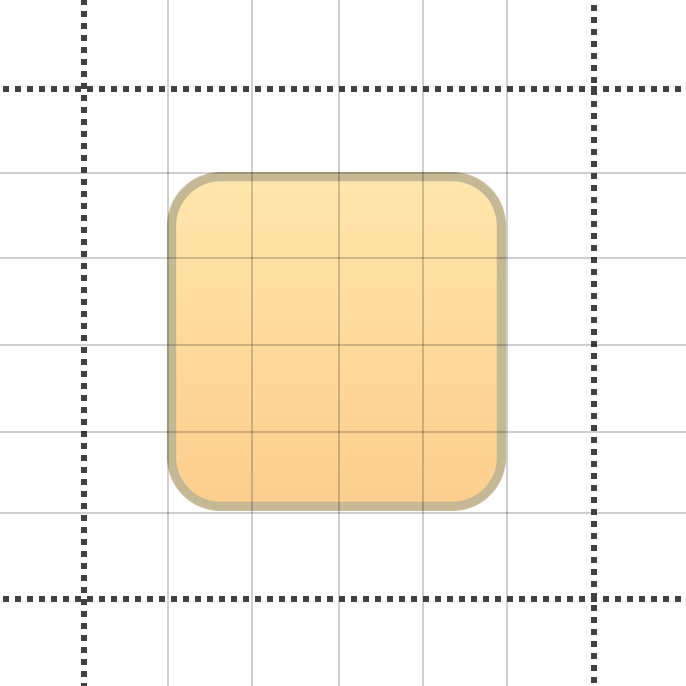
\includegraphics[width=0.25\textwidth]{element_margin_example}
	\caption{Example of element margin}
	\label{fig:element_margin_example}
\end{figure}

\begin{note}
	If margin is used inside a container each element with margin will also be a certain distance from the borders of that specific container. If, for instance, an element has a margin of $10$, then this element would be a distance of $10$ from the borders of the container. This means that there \textit{might} not be need for any padding on the given container.
\end{note}

\subsection{Consistent Margin}
Elements of the same type appearing in the same context must have the same distance to other elements. However, if the elements appear in an order, for example a horizontal list, the first and last element may differ. For instance, the first element may have a smaller left-margin and the last element may have a smaller right-margin. \figref{fig:element_margin_consistency} shows an illustration of this example.

\begin{figure}[h]
	\centering
	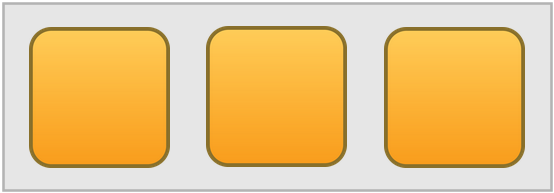
\includegraphics[width=0.45\textwidth]{element_margin_consistency}
	\caption{Example of element margin}
	\label{fig:element_margin_consistency}
\end{figure}


\section{Container Padding}
Each container should provide some padding for its content. This padding should be somewhat identical to the spacing between elements inside the container. \figref{fig:container_padding_example} shows an example of a container with padding. 

\begin{figure}[h]
	\centering
	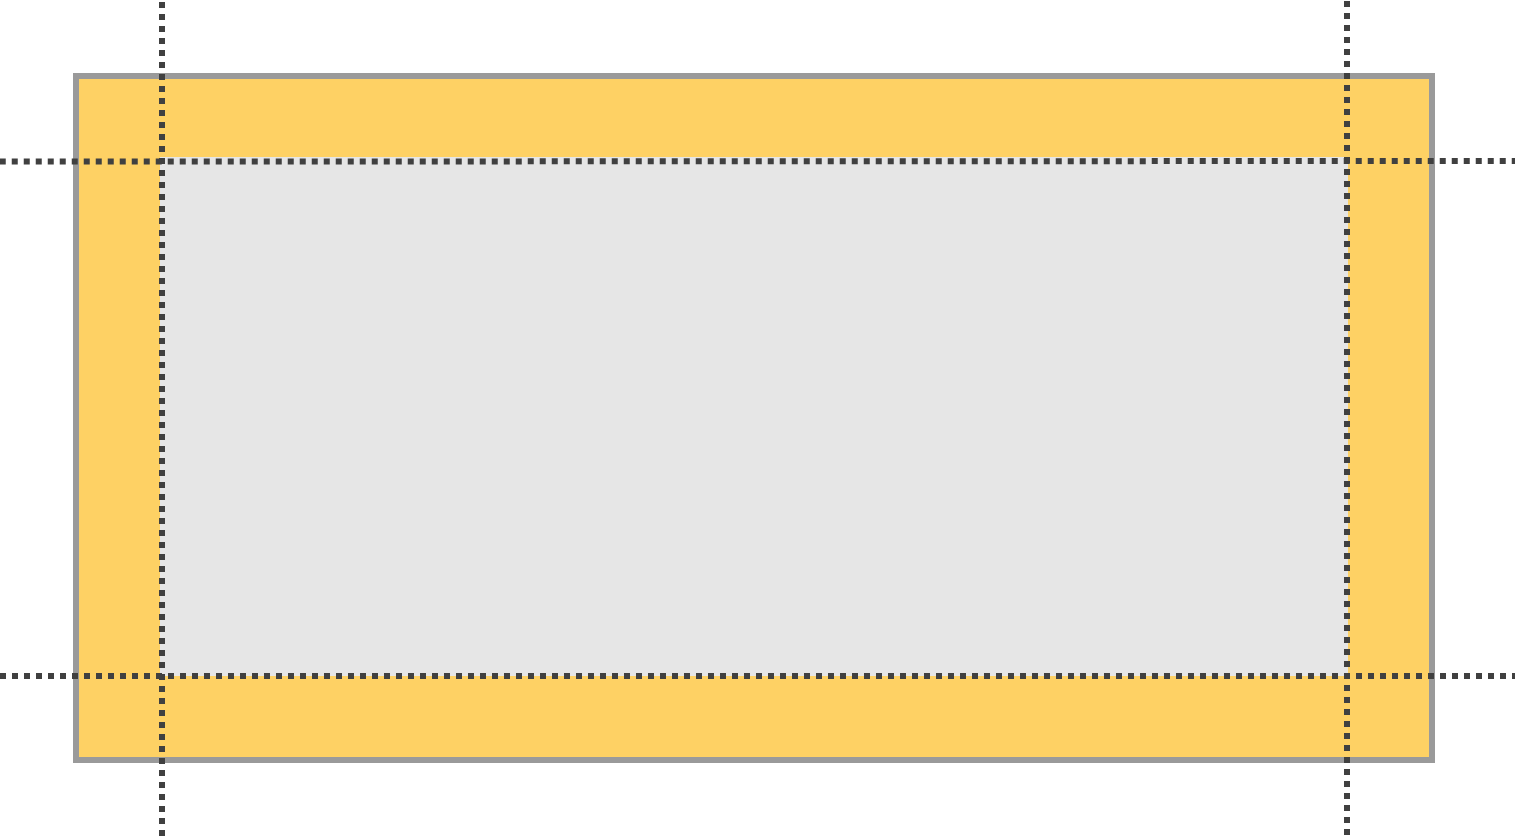
\includegraphics[width=0.65\textwidth]{container_padding_example}
	\caption{Example of a container with padding}
	\label{fig:container_padding_example}
\end{figure}

\begin{note}
	Whenever the content of the container can be scrolled through (for example a \texttt{GridView}) a property called \texttt{clipToPadding} must be set to \texttt{false}. Please refer to the \href{http://developer.android.com/reference/android/view/ViewGroup.html#attr_android:clipToPadding}{Android documentation} for additional information.
\end{note}\todo{The effect of this could be explained more clearly using a figure}


%----------------------------------------------------------------------------------------
%	INDEX
%----------------------------------------------------------------------------------------

\cleardoublepage
\phantomsection
\setlength{\columnsep}{0.75cm}
\addcontentsline{toc}{chapter}{\textcolor{ocre}{Index}}
\printindex

%----------------------------------------------------------------------------------------

\end{document}